\documentclass[11pt]{article}
\usepackage[margin=1in]{geometry}
\usepackage{booktabs}
\usepackage{graphicx}
\usepackage{amsmath,amssymb}
\usepackage[colorlinks=true,linkcolor=loopblue,citecolor=loopblue]{hyperref}
\usepackage[numbers]{natbib}
\usepackage{xcolor}
\definecolor{loopblue}{RGB}{37,99,235}
\definecolor{loopred}{RGB}{220,38,38}
\definecolor{loopgreen}{RGB}{22,163,74}
\definecolor{loopgreenDark}{RGB}{21,128,61}
\definecolor{looporange}{RGB}{234,88,12}
\definecolor{looppurple}{RGB}{124,58,237}
\usepackage{tikz}
\usetikzlibrary{arrows.meta,positioning,shapes.geometric,fit,backgrounds}
% --- Design system tokens (ui-ux-pro-max: Minimal Single Column / Data-Dense) ---
\tikzset{
  loop node/.style={draw, rounded corners=3pt, line width=0.5pt, align=center, font=\small},
  loop circle/.style={draw, circle, line width=0.5pt, align=center, font=\scriptsize},
  loop edge/.style={-{Stealth[length=2.5mm]}, line width=1.0pt, shorten >=1pt, shorten <=1pt},
  loop edge secondary/.style={-{Stealth[length=2.2mm]}, line width=0.6pt, shorten >=1pt, shorten <=1pt},
  loop label/.style={font=\scriptsize, fill=white, inner sep=2pt, rounded corners=1pt},
  loop label small/.style={font=\scriptsize, fill=white, inner sep=1.5pt, rounded corners=1pt},
  loop annotation/.style={font=\scriptsize, text=black!60, align=center},
}
\usepackage{microtype}
\usepackage{array}
\newcolumntype{P}[1]{>{\raggedright\arraybackslash}p{#1}}
\usepackage{tabularx}
\setlength{\emergencystretch}{2em}

\title{The Dynamic Reflexive Loop and the Five Organs:\\[4pt]
\Large A Reflexive Systems Framework from Molecules to Markets\\[6pt]
\normalsize One Loop at Every Scale, Five Organs at Every Level}
\author{Shehzad Ahmed \\ \small Independent University, Bangladesh \\ \small \texttt{github.com/\allowbreak{}shehzadahmed-\allowbreak{}xx/\allowbreak{}mindharness}}
\date{August 27, 2026}

\providecommand{\slash}{}\renewcommand{\slash}{/\allowbreak{}}

\begin{document}
\maketitle

\begin{abstract}
Any system that must act competently under uncertainty, over time, in a world that contains itself, faces the same constraint regardless of substrate. We formalize this constraint as the \emph{dynamic reflexive loop} --- a system whose actions rewrite the conditions for its next actions because the world it acts on contains itself --- and, interpreting Nayebi Cor.~3--5 as five organs, formalize that any stable pattern in such a world must develop them or be exploited by the task distribution that needs them: \textbf{boundary}, \textbf{two-speed memory}, \textbf{salience gate}, \textbf{damping}, and \textbf{internal observer} (our executable interpretation of Nayebi Cor.~3--5, not Nayebi's terminology). The same five, on our reading, appear at every scale we can measure --- from NMDA coincidence detection at the synapse to global workspace competition in the mind to funding invariants in the market. We implement all five as an executable cognitive harness (13 modules, 8 layers, 78/78 tests green) whose audit trail makes each organ separately ablatable, and state for every organ at every scale the specific failure its removal is predicted to produce.
\end{abstract}

%==============================================================================
\section{Introduction: One Loop, Five Organs}
%==============================================================================

Every benchmark score reported for a language model is a pair: weights and the room those weights were tested in. The room contributes more than model generations \citep{lin2026ahe}. The same asymmetry governs minds, markets, and molecules: structure matters more than substrate, and the structure that matters is the same at every scale.

We formalize this structure as the \emph{dynamic reflexive loop}:

\begin{equation}
\mathrm{State}(t) \to \mathrm{harness}(t{+}1) \to \mathrm{State}(t{+}1)
\end{equation}

A system that acts on a world that contains itself, so its actions rewrite the conditions for its next actions. Two channels carry every action outward --- physical (your order executes, calcium floods) and informational (others see you acted and change because of what it meant). When both run, three consequences break normal logic at every scale: models rot from use, measurement corrupts, truth moves.

Any stable pattern in such a world must develop five organs or be exploited (Figure~\ref{fig:fivecycle}):

\begin{figure}[htbp]
\centering
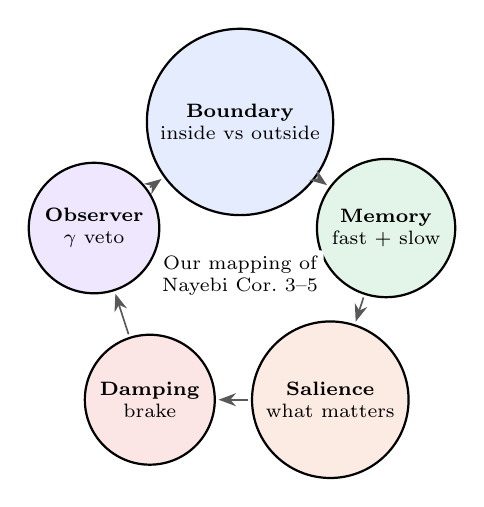
\begin{tikzpicture}[thick]
  \def \r{1.95cm}
  \node[draw, circle, fill=loopblue!12, minimum size=1.50cm, align=center, font=\scriptsize] (b) at (90:\r) {\textbf{Boundary}\\\scriptsize inside vs outside};
  \node[draw, circle, fill=loopgreen!12, minimum size=1.50cm, align=center, font=\scriptsize] (m) at (18:\r) {\textbf{Memory}\\\scriptsize fast + slow};
  \node[draw, circle, fill=looporange!12, minimum size=1.50cm, align=center, font=\scriptsize] (s) at (-54:\r) {\textbf{Salience}\\\scriptsize what matters};
  \node[draw, circle, fill=loopred!12, minimum size=1.50cm, align=center, font=\scriptsize] (d) at (-126:\r) {\textbf{Damping}\\\scriptsize brake};
  \node[draw, circle, fill=looppurple!12, minimum size=1.50cm, align=center, font=\scriptsize] (o) at (162:\r) {\textbf{Observer}\\\scriptsize $\gamma$ veto};
  \draw[loop edge secondary, black!65] (b) -- (m); \draw[loop edge secondary, black!65] (m) -- (s); \draw[loop edge secondary, black!65] (s) -- (d); \draw[loop edge secondary, black!65] (d) -- (o); \draw[loop edge secondary, black!65] (o) -- (b);
  \node[font=\scriptsize, fill=white, inner sep=2pt, rounded corners=1pt, align=center] at (0,0) {Our mapping of\\Nayebi Cor.\ 3--5};
\end{tikzpicture}
\caption{Our mapping of Nayebi Cor.\ 3--5 as a cycle: the warp. Lose one and a task distribution will exploit the gap. Any competent weave must be woven on these five. Nayebi proves abstract pressures; the five-organ labeling is our interpretation.}
\label{fig:fivecycle}
\end{figure}

Selection theorems \citep{nayebi2026} prove abstract selection pressures are mandatory, not optional: low average-case regret \emph{forces} world models, belief-like predictive states, regime-tracking variables (emotion primitives), informational modularity, and representational convergence (Nayebi Thm.~1, 5, Cor.~3--5). We interpret these pressures as requiring our five-organ labeling --- boundary, two-speed memory, salience gate, damping, internal observer --- which is our executable interpretation of Cor.~3--5, not Nayebi's terminology; Nayebi proves the abstract pressures, we map them to the five and implement the mapping as code. We implement all five as an executable harness with an audit trail, so that each organ can be removed independently and the predicted failure checked (\S\ref{sec:falsifiability}).

This paper is the theory paper for that harness. Where our empirical papers \citep{paper-v2-final,paper-v3} test whether the witness makes an LLM honest, this paper asks why the witness is one of five, why the five appear at every scale, and what it would mean if the universe, as the largest loop, also needs them.

\subsection*{Three frameworks in one paragraph each --- for the new reader}

\textit{Global Workspace Theory (GWT, Baars 1988; Dehaene \& Changeux 1998--2004):} Consciousness is the global availability of information. Specialized processors (vision, memory, affect, planning) compete to get their content into a limited-capacity workspace; the winner is broadcast to every other processor and thereby becomes conscious \citep{baars1997,atallah2026gwt}. Baars's theater metaphor: the workspace is the stage, processors are the audience, attention is the spotlight, and consciousness is what is on stage. Dehaene's neuronal workspace adds reverberant fronto-parietal loops as the neural substrate \citep{atallah2026gwt}. If you have never read GWT, read Baars (1997, \emph{In the Theatre of Consciousness}) and Dehaene et al.\ (1998, \emph{Proc.\ Natl.\ Acad.\ Sci.}) --- 30 pages total, and you will have the framework. In our terms, GWT is Layer 4: coalition competition $\to$\allowbreak{} winner broadcast, experienced as ``my thought'' 200\,ms after. Our contribution is to make the broadcast checkable (ledger) and to measure whether the winner was worth broadcasting ($\gamma$).

\textit{Predictive processing / active inference (Friston, Clark, Seth):} Perception is not input $\to$\allowbreak{} processing $\to$\allowbreak{} experience. It is prediction $\to$\allowbreak{} error $\to$\allowbreak{} corrected prediction $\to$\allowbreak{} experience \citep{seth2021,clark2016surfing}. The brain predicts the next moment and corrects by prediction error; affect is interoceptive prediction (what the body will need next); attention is precision weighting (which errors to trust). Seth's ``controlled hallucination'' and ``beast machine'' locate selfhood in control-oriented interoceptive inference: the feeling of being alive is the prediction of the body's viability, felt before the need \citep{seth2021}. If you have never read predictive processing, read Seth (2021, \emph{Being You}, ch.~2--4) or Clark (2016, \emph{Surfing Uncertainty}, ch.~3) --- the harness implements the same loop in code. In our terms, predictive processing is the salience gate and the observer at the scale of felt presence.

\textit{Selection theorems (Nayebi, UAI 2026, 23 pages):} Classical results show optimal control \emph{can be implemented} using world models or belief states, but not that they are \emph{required}. Nayebi proves they \emph{are} required --- quantitatively, with regret bounds, without assuming optimality or determinism, in fully and partially observed settings \citep{nayebi2026}. Their method reduces prediction to binary betting; low average-case regret forces the agent to have made the right bets often enough to have implicitly learned the transition kernel, belief states, and regime trackers. If you have never read selection theorems, read Nayebi (2026, arXiv:2603.02491, 23 pages, 1 figure) --- the harness's five are Corollaries~3--5 of that paper, and every ``Why necessary'' paragraph in \S\ref{sec:organs} is a corollary made executable. In our terms, selection is why the five are the warp, not the weft.

\subsection*{Research questions}

\begin{center}
\setlength{\tabcolsep}{3pt}
\small
\begin{tabular}{p{0.85cm}p{5.45cm}p{5.45cm}}
\toprule
 & Question & Hypothesis \\
\midrule
RQ1 & What must any stable reflexive system have? & Five organs: boundary, two-speed memory, salience gate, damping, internal observer (Nayebi Cor.\,3--5). \\
RQ2 & Can the five be built as a runnable harness with an audit trail? & Yes: 11 modules, 8 layers, 78/78 tests green, every hop cause-signed. \\
RQ3 & Do the five appear at every scale? & Yes: molecule $\to$\allowbreak{} universe, same five at 8 levels, each loop with its own literature. \\
RQ4 & Is the decomposition arbitrary? & Not obviously: independent observational taxonomies reach broadly similar distinctions (\S\ref{sec:traditions}) --- weak support only, and no claim rests on it. \\
RQ5 & What about the universe as the largest loop? & If the five are required at every measured scale, the universe may also need them. We ask, not claim. \\
\bottomrule
\end{tabular}
\end{center}

\subsection*{Roadmap}

\S\ref{sec:lit-review} reviews eight literatures that converge on the same five. \S\ref{sec:loop} defines the dynamic reflexive loop (reflexivity, its three consequences, and how the loop expands). \S\ref{sec:three-sides} shows reality, perception, and self as one loop's three sides. \S\ref{sec:organs} proves the five, each fully at every level with what happens without it. \S\ref{sec:levels} shows how the eight levels nest (each level's broadcast is the next level's input). \S\ref{sec:traditions} notes prior observational taxonomies as historical context, and \S\ref{sec:universe} states why we stop at the market rather than extending to cosmology. \S\ref{sec:choice} gives the only real choice, and \S\ref{sec:what-it-all-means} synthesizes what it all means. A new reader can read front-to-back; each section's opening tells you what it proves and each section's close tells you the takeaway.

\subsection*{Key terms (one sentence each)}

\begin{center}
\setlength{\tabcolsep}{3pt}
\small
\begin{tabular}{p{3.0cm}p{9.05cm}}
\toprule
Term & Plain English + one example \\
\midrule
Reflexive loop & System acts on a world that contains itself, so the next input already contains the last act. \emph{Example:} you believe a stock will rise $\to$\allowbreak{} you buy $\to$\allowbreak{} price rises because you bought. \\
Boundary & What counts as inside vs outside --- selectively permeable, not a wall. \emph{Example:} ledger's source tag (memory\_lookup vs model\_prior). \\
Two-speed memory & Fast labile (one-shot, episodic) + slow structural (statistical, semantic) + sleep as the save. \emph{Example:} hippocampus today, cortex over weeks. \\
Salience gate & What gets tagged for consolidation --- vivid, emotional, surprising wins. \emph{Example:} AffectState [0.5,2.0] shifting the next bid. \\
Damping & What prevents runaway --- brake on positive feedback. \emph{Example:} LTD pulling AMPA out, or \texttt{cull\_failed} deleting a below-rate skill. \\
Internal observer & Slower loop watching faster one, veto-able; $\gamma$ = changed/diagnosed (Stage 1: always-on anomaly scoring, cheap; Stage 2: triggered diagnosis, expensive). \emph{Example:} ledger check before the next claim; compliance guard $\gamma=0$ proves inert watching. \\
$\gamma$ & changed / diagnosed --- the only honest measure of whether the observer steered. \emph{Example:} $\gamma=0$ (compliance guard, always-no) watches perfectly, never steers; $\gamma>0$ (active gate) changed the trajectory. \\
Warp / weft & Warp = five mandatory threads (Nayebi Cor.\,3--5); weft = your design woven on them \citep{nayebi2026}. \emph{Example:} harness is one weave, Cordis is the loom; change weft, same warp, different mind. \\
S126 & Attribution battery: handed vs generated text, 98\% confidence on fabrications vs 87\% on truths (more confident about lies). \emph{Example:} model claims it generated what it was handed. \\
Light$\to$\allowbreak{}Deep & Consolidation pipeline: Light (dedupe) $\to$\allowbreak{} REM (concept extract) $\to$\allowbreak{} Counterfactual (variant$\to$\allowbreak{}simulate$\to$\allowbreak{}regret) $\to$\allowbreak{} Deep (promote if $\geq$2 query types) \citep{tononi2014}. \emph{Example:} REM ablation is dream-deprivation. \\
Barzakh & Any realm that connects two opposites while keeping them separate (Ibn Arabi). \emph{Example:} the now between past and future. \\
Autopoiesis & Bounded network that produces the very components that maintain it \citep{maturana1980}. \emph{Example:} metabolism $\to$\allowbreak{} lipids $\to$\allowbreak{} membrane $\to$\allowbreak{} metabolism. \\
\bottomrule
\end{tabular}
\end{center}

\begin{figure}[htbp]
\centering
\fbox{\parbox{0.92\textwidth}{\small
\textbf{One turn, five organs, 30 seconds --- walk one input through the harness.} Prompt: ``Summarize the close.''

\textit{Boundary:} \texttt{ProvenanceLedger.bind()} tags the prompt as external-tool vs the model's prior output as model\_prior; output spans carry the tag. Without the ledger, the next turn cannot tell what it was handed from what it generated.

\textit{Two-speed memory:} The turn's episodic MemoryItem (query\_hits for this prompt) is staged; at night, Light dedupes, REM extracts, Counterfactual simulates otherwise, Deep promotes if $\geq$2 query types. Without two speeds, new overwrites old.

\textit{Salience gate:} AffectState (valence/arousal) multiplies the prompt's bid before the workspace competition; high salience amplifies the winner. Without the gate, every trace equally promoted.

\textit{Damping:} \texttt{cull\_failed} deletes below-rate skills; Light dedup merges near-identical traces. Without damping, one coalition wins forever.

\textit{Internal observer:} MonitorGate Stage 1 scores anomaly; if triggered, Stage 2 diagnoses $\to$\allowbreak{} trust/retry/revise/abstain, $\gamma$ = changed/diagnosed. Without the observer, beautiful reports, zero steering.

One input, five organs, one turn. The next turn's harness is already different: ledger has one more binding, memory has one more episodic item, affect has shifted, and the observer has scored whether watching steered.
}}
\caption{One turn through the five organs --- concrete walkthrough for the new reader. Every forward reference in the paper (ledger, $\gamma$, Light$\to$\allowbreak{}Deep, AffectState) is anchored here before its formal definition. \S\ref{sec:traditions} is historical context and can be skipped without breaking this flow.}
\label{fig:oneturn}
\end{figure}

%==============================================================================
\section{Literature Review}
\label{sec:lit-review}
%==============================================================================

We review eight literatures that converge on the same five, from different instruments, in different languages, on the same constraint. Each could be its own review; here we give the loop each literature found, fully, with the science that makes it checkable. Read this section as reference --- the loop definition (\S\ref{sec:loop}) and the boxed figure above give you enough to follow the argument; return here for depth on any literature.

\subsection{Synaptic plasticity: Hebb in protein, BCM, and the need for damping}

Hebbian plasticity --- cells that fire together wire together --- was long studied as long-term potentiation (LTP, persistent strengthening) and long-term depression (LTD, persistent weakening), both activity-dependent, input-specific, and lasting hours \citep{tononi2014}. At the synapse, NMDA is Hebb's law in protein: a coincidence detector needing glutamate (pre) and depolarization (post, Mg$^{2+}$ ejected, plus glycine), opening only when pre and post fire together. High Ca$^{2+}$ spikes (big, brief) drive CaMKII Thr286 bistable switching and AMPA insertion (LTP); low Ca$^{2+}$ trickles drive calcineurin$\to$\allowbreak{}PP1 and AMPA removal (LTD) \citep{tononi2014}. Spike-timing-dependent plasticity (STDP) refines this to causal timing: pre-before-post strengthens, post-before-pre weakens \citep{bipoo1998}.

Hebbian plasticity alone is a positive-feedback process that destabilizes networks: LTP and LTD, left unchecked, let one synapse take all strength \citep{tononi2014}. Stabilization requires a second, slower process operating at a different timescale than STDP \citep{tononi2014}: the Bienenstock-Cooper-Munro (BCM) sliding threshold \citep{bienenstock1982}. At the molecular scale, this is already autopoiesis in miniature: Maturana and Varela's bounded network of processes that produces the very components that maintain the system \citep{maturana1980} --- metabolism creates proteins that regenerate the cell wall that preserves the environment for metabolism. Nobel laureate Eric Kandel and Michael Merzenich showed the same loop at circuit scale: adult cortical map reorganization via experience-driven gene transcription and myelin thickening \citep{kandel2001,merzenich1984}. Perineuronal nets write-protect. The lesson for any reflexive system is already here: potentiation (learning) without damping (forgetting/scaling) is seizure, not memory.

\subsection{Sleep, synaptic homeostasis, and two-speed consolidation}

Sleep is not rest. It is a second, offline computation that corrects what wake did. The synaptic homeostasis hypothesis (SHY) proposes that wake's net potentiation (learning throughout the brain) increases cellular needs, energy cost, and saturation, and must be renormalized during sleep via global downscaling --- multiply all synapses by $<1$, keep relative strengths, delete noise --- to restore selectivity \citep{tononi2014}. During slow-wave sleep, the brain goes offline so renormalization via depression can happen without corrupting nondeclarative skills that would be corrupted if new learning occurred during sleep without environmental feedback \citep{tononi2014}. Hippocampal replays of previously encoded patterns during slow oscillations mediate stabilization and gradual integration of declarative memory into cortex \citep{tononi2014}.

The active system consolidation hypothesis adds replay: repeated reactivations in hippocampus during slow oscillations stabilize and integrate memory \citep{tononi2014}. The memory function of sleep requires both non-REM and REM; targeted memory reactivation (TMR) shows cuing during sleep strengthens traces only if cued memories relate to prior knowledge \citep{tononi2014}. At harness scale, this is Light$\to$\allowbreak{}REM$\to$\allowbreak{}Deep: downscale, extract, simulate otherwise, promote if $\geq$2 query types. REM ablation is dream-deprivation made executable.

\subsection{Predictive processing, interoception, and the beast machine}

Predictive processing reframes perception as controlled hallucination: the brain predicts the next moment and corrects by prediction error, with affect arriving before the need \citep{seth2021,clark2016surfing}. Seth's interoceptive inference extends this inward: emotions are not reactions to perception but predictions \emph{about} perception, made before perception arrives --- valence/arousal as the brain's assessment of regulatory success, felt as gain that shifts every downstream bid \citep{seth2021}. Interoception (heartbeat, blood pressure, gut tension) is not an add-on to exteroception. It is the foundation --- the brain's first job is to keep the body alive; everything else is built on allostasis \citep{seth2021,clark2016surfing}.

Hohwy and Seth provide the systematic basis for identifying neural correlates of consciousness within predictive processing \citep{seth2021}, while Seth's ``beast machine'' locates selfhood in control-oriented interoceptive inference: pleasure, pain, and desire as self-annihilating free-energy gradients via interoceptive active inference \citep{seth2021}. In our terms, this is the salience gate and the internal observer at the scale of felt presence --- regime-tracking variables that tell every specialist which world they're in, and the slower loop that watches whether the prediction that contains the predictor was correct.

\subsection{Global workspace and conscious access}

Global Workspace Theory (GWT), introduced by Baars (1988) and extended by Dehaene and Changeux as the Global Neuronal Workspace (GNW), proposes that consciousness is the global availability of information: information becomes conscious when simultaneously made available to a wide range of localized, subpersonal processes jointly comprising a workspace \citep{baars1997,atallah2026gwt}. Baars's theater metaphor and Dehaene's neuronal instantiation agree: a considerable amount of processing is possible without consciousness, attention is a prerequisite, and consciousness is required for specific tasks \citep{baars1997,atallah2026gwt}. The GNW hypothesis synthesizes these as a defined fronto-parietal network of reverberant loops enabling access to a wider array of modular processors \citep{atallah2026gwt}.

Fifty years of GWT research now emphasizes transient resonant neurodynamics, prefrontal function, and meditation-related characterizations \citep{baars1997}, with self-organized criticality as a framework for the workspace's dynamics \citep{baars1997}. In our harness, the workspace is Layer 4: coalition competition (salience $\times$ utility, modulated by AffectState [0.5,2.0]), winner broadcast globally, experienced as ``my thought'' 200\,ms after the competition resolved. Gazzaniga's interpreter, Johansson's choice blindness, and Nisbett \& Wilson's verbal reports are the same failure without a ledger: the narrator wins after the action and explains as if it decided \citep{gazzaniga2000,johansson2005,nisbett1977}.

\subsection{Metacognition, confidence, and the $\gamma$-gate}

Metacognition --- thinking about thinking --- is not one thing but two, dissociable in humans and in silicon: Type-1 performance (discrimination) and Type-2 sensitivity (knowing whether you were correct), neurally distinct and formally separable via signal detection theory \citep{cacioli2026,maniscalco2012}. Maniscalco and Lau's meta-$d'$ framework quantifies this: given the observed confidence $\times$ accuracy contingency table, find the $d'$ an ideal observer would need to produce the observed Type-2 hit and false-alarm rates (Hautus log-linear correction for degenerate cells), bias-free unlike confidence-accuracy correlation \citep{maniscalco2012,cacioli2026}. Their method, extended hierarchically (HMeta-d), shows metacognitive efficiency is domain-specific, dissociable from Type-1, and neurally distinct \citep{cacioli2026}.

Fleming's synthesis (Annual Review of Psychology, 2024) and the MetaLab program systematize this: metacognition and confidence as reviewable constructs with signal-detection-theoretic models \citep{fleming2024}. In LLMs, the same framework applies without claiming phenomenology: meta-$d'$ measures whether confidence tracks accuracy, with functional parallels to human metacognition but not mechanistic identity \citep{cacioli2026}. Cacioli et al. show intermediate-layer signal present even when final layers suppress the report --- introspection is underelicited, not absent \citep{cacioli2026}. Cao et al. show wiring monitoring into control yields +8.6 percentage points --- monitoring that steers vs monitoring that merely reports \citep{cao2026}. Macar et al. show refusal-direction ablation improves detection +53 points and a trained bias vector +75 points, both without increasing false positives \citep{macar2026}. Our $\gamma$ (changed/diagnosed) is the harness's operationalization (Figure~\ref{fig:gammagate} shows the two stages and the compliance guard): Stage 1 (cheap, always-on anomaly from error rate, failure streak, embodied strain) and Stage 2 (triggered diagnosis $\to$\allowbreak{} trust/retry/revise/abstain), with compliance guard as $\gamma=0$ negative control proving inert watching.

\subsection{Selection theorems and the warp}

Nayebi (UAI 2026, 23 pages) proves quantitative selection theorems: strong task performance (low average-case regret) \emph{forces} world models, belief-like memory, and --- under task mixtures --- persistent regime-tracking variables resembling functional emotion primitives, plus informational modularity under block-structured tasks \citep{nayebi2026}. Their method reduces predictive modeling to binary betting decisions; regret bounds limit probability mass on suboptimal bets, enforcing predictive distinctions. In fully observed settings this yields interventional transition kernel recovery; under partial observability it implies necessity of predictive state and belief-like memory, resolving Richens et al. (2025) \citep{nayebi2026}. This is why the harness's five are the warp: any competent weave must be woven on them, or a task distribution will exploit the gap.

\subsection{Autopoiesis and the reflexive self: the loop that builds itself}

Two literatures name the same loop that the previous six describe as mechanism. Maturana and Varela's autopoiesis defines a bounded network of processes that produces the very components that maintain the system: metabolism creates proteins and lipids that regenerate the cell wall that preserves the environment for metabolism --- the product of the system is the system itself \citep{maturana1980}. This is the first reflexive loop at the scale of life, and every larger loop is the same, at a different scale. Anthony Giddens's reflexive project of the self \citep{giddens1991} describes the same loop at the scale of a life: in modernity, human life becomes an open feedback loop where we observe our behaviors, ingest knowledge about ourselves from expert systems, and chronically revise our actions, which alters the social structure we exist within. Together, the biopsychosocial loop: autopoiesis at the cell, neuroplasticity (LTP $\to$\allowbreak{} myelination) at the circuit, reflexive self-monitoring at the person --- one loop, three names, same structure: bounded, self-producing, self-revising, where the product is the producer.

\subsection{Observational taxonomies of mind}

Contemplative traditions produced detailed taxonomies of mind from sustained first-person observation, and some of their distinctions correspond loosely to the organs described here (\S\ref{sec:traditions}). We treat this as historical context rather than as support: the correspondences are ours and are not load-bearing.

\subsection{Agentic harness engineering and the loom}

Agentic Harness Engineering (AHE, Lin et al. 2026) lifts Terminal-Bench pass@1 from 69.7\% to 77.0\% on frozen base models via observability-driven evolution of harness components, with component ablations localizing gains to tools, middleware, and long-term memory --- system-prompt edits alone regress \citep{lin2026ahe}. Cross-family transfer ($+5$ to $+10$pp without re-evolution) proves the mind is in the harness, not just the weights. The 2026 survey landscape confirms this at scale: Awesome-Agent-Harness catalogs 110+ papers and 23 systems, with Vercel's reported finding that removing 80\% of tools helped more than any model upgrade --- the harness, not the weights, is the bottleneck. CodeAct outperforms on 17/17 Mint benchmarks with 20\% fewer turns; Schema First shows interface design alone is insufficient without semantic discipline \citep{lin2026ahe}. Memory surveys (Hu et al. 2025, Luo et al. 2026, Tang et al. 2026) proliferate but none organize around security as primary axis, underscoring that the witness (provenance, audit trail) remains the missing invariant in most harnesses.

DeepSeek Harness (Cordis) provides the loom: a kernel that mounts/unmounts plugins as reversible effects, profile-composable. Our contribution is the opinionated weave: five invariants as mandatory warp, each as a Cordis plugin with a metric (coverage, $\gamma$, dedup ratio, skill survival, dissolution progress), plus the audit trail that converts analogy into measurement (Appendix~\ref{app:cordis}). Where AHE evolves the harness automatically, we specify \emph{which} harness patterns must transfer (the five) and how to measure whether each re-tie helped.

%==============================================================================
\section{The Dynamic Reflexive Loop}
\label{sec:loop}
%==============================================================================

\subsection{Reflexivity: the map becomes the territory}

Most systems in textbooks are open: archer $\to$\allowbreak{} target. Archer aims, target sits still. You can measure without disturbing, learn the rule once, keep using it.

Reflexive systems add one arrow back. Figure~\ref{fig:oneloop} shows the loop that replaces the open-system archer.

\begin{figure}[htbp]
\centering
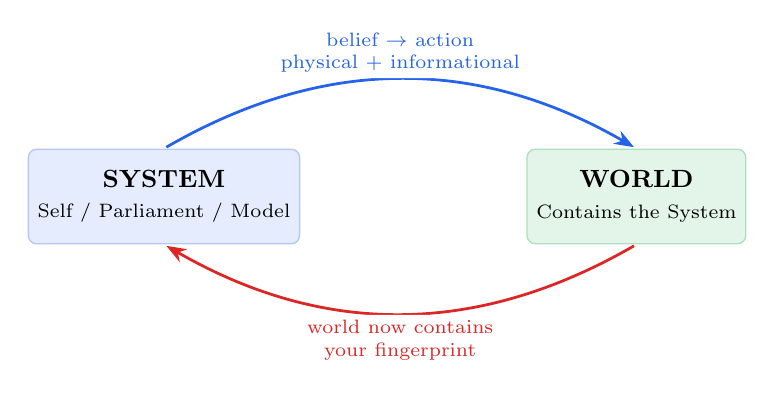
\begin{tikzpicture}[thick]
  \node[draw, rounded corners=3pt, fill=loopblue!12, draw=loopblue!35, line width=0.5pt, minimum width=2.6cm, minimum height=1.2cm, align=center, font=\small] (sys) at (0,0) {\textbf{SYSTEM}\\\scriptsize Self / Parliament / Model};
  \node[draw, rounded corners=3pt, fill=loopgreen!12, draw=loopgreen!35, line width=0.5pt, minimum width=2.6cm, minimum height=1.2cm, align=center, font=\small] (world) at (6,0) {\textbf{WORLD}\\\scriptsize Contains the System};
  \draw[-{Stealth[length=2.5mm]}, loopblue, line width=1.0pt, shorten >=1pt, shorten <=1pt] (sys.north) to[out=30,in=150] node[midway, above, loop label, align=center] {belief $\to$\allowbreak{} action\\physical + informational} (world.north);
  \draw[-{Stealth[length=2.5mm]}, loopred, line width=1.0pt, shorten >=1pt, shorten <=1pt] (world.south) to[out=-150,in=-30] node[midway, below, loop label, align=center] {world now contains\\your fingerprint} (sys.south);
\end{tikzpicture}
\caption{The one loop: System acts on a World that contains the System, so the World the System next perceives already contains the System's last act. Two channels (physical + informational), three consequences (models rot, measurement corrupts, truth moves).}
\label{fig:oneloop}
\end{figure}

\begin{equation}
\begin{aligned}
\text{Self}(t) &\xrightarrow{\text{acts}} \text{World}(t) \text{ that now contains Self}(t)\text{'s act} \\
\text{Self}(t{+}1) &\neq \text{Self}(t) \xrightarrow{\text{perceives}} \text{World}(t{+}1) \neq \text{World}(t)
\end{aligned}
\end{equation}

No fixed point. Only the loop, always becoming, never returning.

Two channels always run: \textbf{physical} (your order executes, muscles move, calcium floods) and \textbf{informational} (others see you acted and change because of what it meant, the network updates routing, the market reprices). When both run, cause and effect tangle.

\subsection{Three consequences that break normal logic}

When both channels run, three consequences follow that break the logic that works for open systems:

\textbf{1. Models rot from use.} An arbitrage edge exists because no one trades it. Trade it and it vanishes. Your knowledge is consumed by acting on it. Chess openings stay good; market patterns don't. At the synapse: a coincidence detector used without error correction strengthens spurious correlations until it fires for everything.

\textbf{2. Measurement corrupts.} Goodhart: when a measure becomes a target, it ceases to be a good measure. Hospital waiting times $\to$\allowbreak{} patients parked in ambulances. Synapse firing rates $\to$\allowbreak{} homeostasis breaks. Benchmark scores without a witness $\to$\allowbreak{} model learns to produce the score without the reasoning.

\textbf{3. Truth moves.} Bank run: ``bank will fail'' $\to$\allowbreak{} withdraw $\to$\allowbreak{} bank fails --- belief made itself true. Synapse: ``this input predicts that output'' $\to$\allowbreak{} strengthen $\to$\allowbreak{} now it does, even if initially spurious. No fixed truth to converge on --- only temporarily stable consensus that your own actions keep perturbing.

This is Soros's two functions running at once: cognitive (understand reality) + manipulative (change reality). When both run, neither yields a determinate answer. Humans add a third: self-observation is also an action. Labeling yourself ``anxious'' installs a filter that recruits confirming evidence. Introspection writes on what it reads. Autopoiesis formalized this: you are a network whose products regenerate the conditions for their own production.

\subsection{The expanding loop: Self(t) contains Self(t-1)}

When the loop \emph{is} the self --- not a loop the self has, but the self that the loop is --- and it is expanding, each iteration is larger in \emph{reach}, not size: Self(t+1) contains Self(t) as memory, plus the world Self(t) changed, plus the prediction of what Self(t+1) will do. The loop spirals, never returns (Figure~\ref{fig:expanding}).

At the synapse: Ca$^{2+}$ $\to$\allowbreak{} CaMKII Thr286 $\to$\allowbreak{} more AMPA $\to$\allowbreak{} stronger next Ca$^{2+}$, each coincidence making the next more likely. Tag-and-capture gives proteins to what was already strong. At the mind: coalition wins $\to$\allowbreak{} broadcast $\to$\allowbreak{} biases next vote $\to$\allowbreak{} rehearsed $\to$\allowbreak{} myelinated (100$\times$ speed) $\to$\allowbreak{} highway. At the person: act $\to$\allowbreak{} world contains your act $\to$\allowbreak{} different you perceives different world $\to$\allowbreak{} loop widens.

The trap and the freedom are the same mechanism: worry practiced 1,000 times is one worry amplified 1,000 times by its own winning. You don't choose whether to feed the loop. Only what you feed it.

\begin{figure}[htbp]
\centering
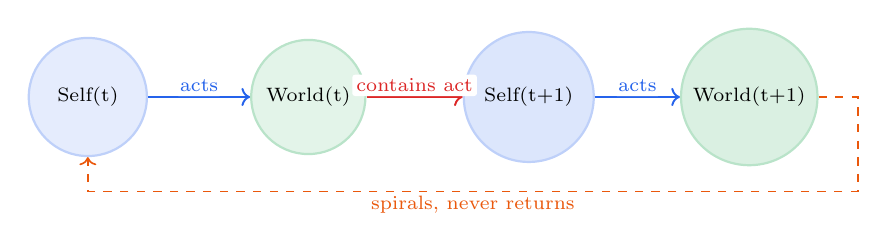
\begin{tikzpicture}[thick, every node/.style={font=\scriptsize}]
  \node[draw, circle, fill=loopblue!12, draw=loopblue!30, minimum size=1.50cm, align=center] (s0) at (0,0) {Self(t)};
  \node[draw, circle, fill=loopgreen!12, draw=loopgreen!30, minimum size=1.45cm, align=center] (w0) at (2.8,0) {World(t)};
  \node[draw, circle, fill=loopblue!16, draw=loopblue!30, minimum size=1.65cm, align=center] (s1) at (5.6,0) {Self(t+1)};
  \node[draw, circle, fill=loopgreen!16, draw=loopgreen!30, minimum size=1.55cm, align=center] (w1) at (8.4,0) {World(t+1)};
  \draw[->, loopblue, line width=0.7pt] (s0) -- node[above, loop label small] {acts} (w0);
  \draw[->, loopred, line width=0.7pt] (w0) -- node[above, loop label small] {contains act} (s1);
  \draw[->, loopblue, line width=0.7pt] (s1) -- node[above, loop label small] {acts} (w1);
  \draw[->, looporange, line width=0.6pt, dashed] (w1.east) -- ++(0.5,0) -- ++(0,-1.2) -| (s0.south) node[pos=0.25, below, loop label small] {spirals, never returns};
\end{tikzpicture}
\caption{The expanding reflexive loop: Self(t) contains Self(t-1) as memory, plus the world Self(t) changed. The loop spirals wider each turn, never returning. Self(t+1) $\neq$ Self(t), World(t+1) $\neq$ World(t).}
\label{fig:expanding}
\end{figure}

\subsection{Selection describes succession, not power}
\label{sec:occasionalism}

One clarification matters for how every claim below should be read. Selection
theorems do not show that the five organs \emph{cause} low regret. They show
that systems which are \emph{followed by} low regret, under mixed tasks over
time, turn out to have them --- and that systems lacking one are exploited by
the task distribution that needs it \citep{nayebi2026}. Selection is a filter
on what persists, not a mechanism that pushes. We therefore state results
throughout as regularities (``where the ledger is checked, attribution accuracy
is higher'') rather than as causal powers of the components, and the audit
trail records the succession so the regularity can be checked rather than
assumed.

%==============================================================================
\section{Reality, Perception, and Self as One Loop Seen from Three Sides}
\label{sec:three-sides}
%==============================================================================

Reality, perception, and self are not three topics. They are one reflexive loop seen from three sides. We take each side in turn, with the science that makes it checkable.

\subsection{Reality as it looks from outside: the constraint space}

What we call reality is not a thing but \emph{what stable looping looks like when it has the five organs} \citep{maturana1980,tononi2014}. The substrate --- matter, energy, information --- is what the loop is made of the way a wave is made of water: necessary, but not what the wave is. What the wave is is the looping. A universe where the five are required for persistence looks exactly like ours: full of bounded, learning, prioritizing, self-correcting patterns, each temporarily stable, each constructed, each maintained, each doomed to dissolve when the relations that make it this pattern scatter.

Reality at this level is: what counts as inside vs outside is not given. It is \emph{maintained} --- the membrane is produced by the network it bounds (autopoiesis \citep{maturana1980}), the ledger is bound every turn or claims float free, the legal entity is re-asserted or risk socializes. At every scale from lipid bilayer (selectively permeable to glucose, not to enzymes) to peripersonal space (``this hand is mine'' vs rubber-hand illusion) to Provenance Ledger (every span source-bound + ref, coverage 1.000 in both living sessions), the boundary is not a wall built once. It is a permeability maintained at each instant, or no pattern persists. Connectomics confirms the same: having every wire for forty years (\emph{C.~elegans} 302 neurons since 1986 \citep{white1986} $\to$\allowbreak{} fly 140,000 in 2023 \citep{dorkenwald2023}) still doesn't predict behavior, because behavior lives in dynamics, not topology --- exactly the five, not the wiring.

\subsection{Perception as it looks from inside, predicting outward}

Perception is a controlled hallucination --- the brain's prediction, constrained by sensory error \citep{seth2021,clark2016surfing}. This inverts the textbook:

Perception is not input $\to$\allowbreak{} processing $\to$\allowbreak{} experience. It is prediction $\to$\allowbreak{} error $\to$\allowbreak{} corrected prediction $\to$\allowbreak{} experience \citep{seth2021}. The prediction comes first; sensory input is the \emph{correction}, not the source. You hallucinate the next moment and the world reins it in --- more or less, depending on precision weighting \citep{clark2016surfing}. Affect as interoceptive prediction arrives as feeling before the need --- valence/arousal as the brain's assessment of regulatory success, broadcast as gain that shifts every downstream bid \citep{seth2021,sofroniew2026}. Attention as precision weighting estimates which errors to trust --- high precision on visual error means ``trust the eyes,'' high on interoceptive means ``trust the gut'' \citep{clark2016surfing}. The now as a 200--500\,ms window stitched after the fact and backdated --- postdictive masking, flash lag, color phi all prove the brain waits, lets what comes \emph{after} change what was experienced \emph{before}, then seals the window and stamps ``now'' \citep{libet1983,wegner2002}. What you experience as now already contains the future that revised it.

The world you perceive is the winning prediction being broadcast --- the hallucination that survived error correction, made globally available \citep{baars1997,atallah2026gwt}, experienced as found. Not true. Viable. The difference is the whole point of allostasis: the system doesn't need to know what is true. It needs to keep essential variables within bounds \citep{seth2021}. Knowing is a side effect of staying alive long enough to predict well.

In the harness: perception is one bidder among many, proposing ``what is happening'' with a salience bid. The workspace competition decides which perception wins the broadcast. The ledger records where the winner came from. Without the ledger, the winning prediction is experienced as ``the way things are.'' With the ledger, it is experienced as ``the prediction that won, from this source, with this confidence'' --- checkable, not found.

Each strand here has its own literature: controlled hallucination \citep{seth2021,clark2016surfing}, precision weighting \citep{clark2016surfing}, the postdictive construction of the now \citep{libet1983,wegner2002}, interoceptive inference \citep{seth2021}, and global broadcast \citep{baars1997,atallah2026gwt}.

\subsection{Self as it looks from inside, predicting itself}

Self is the hallucination that hallucinates itself --- the prediction of the predictor, maintained and presented as found. Three selves, usually confused as one, each a paper:

\textit{Minimal self} --- ``this body is mine'' --- interoception, proprioception, peripersonal space; the prediction of where the body is and what is within reach. Built from the same predictive machinery as perception but turned inward. Survives even when narrative collapses (depersonalization: story dissolves, body boundary remains). Fails in rubber-hand illusion (synchronous touch updates hand-location prediction), succeeds in skin. This is Seth's foundation: selfhood as allostatic prediction, the feeling of being alive that is the basis for all the rest \citep{seth2021}. In the harness: EmbodiedState + peripersonal boundary, affordance space as what appears as possible before the parliament votes.

\textit{Narrative self} --- ``who I am over time'' --- cause-signed SelfModelService, CAS-revisioned (N $\to$\allowbreak{} N+1 or rejected), three cause channels (action-outcome vs narrative-summary vs external-write, so narrated traits cannot file as lived ones), verbatim-archived, diffable, re-injected every turn or drifts $>$30\% in 12 turns \citep{choi2024}. The press secretary that wins \emph{after} the action and explains as if it decided \citep{gazzaniga2000,johansson2005,nisbett1977}. It doesn't lie. It confabulates the most coherent story where ``I'' did it, with complete confidence, because that is what pattern completion does when it only has the broadcast \citep{lindsey2025,macar2026}. Real the way a rainbow is real: photographable, navigable, causal, but no thing at a location.

\textit{Social self} --- ``who we think I am'' --- built from others' predictions of you, which you internalize and then predict yourself through. Language externalizes the witness --- writing as ledger outside the skull where the loop can be audited by others, not just by the slower watcher inside. This is the informational channel of reflexivity: not just that actions perturb the physical world, but that actions change what others predict you will do.

All three are currently winning coalitions, not a captain. No homunculus. Only speed ratios: slower loops vetoing faster ones. Self is not the thinker. It is the broadcast of the winner, experienced as ``I,'' maintained by re-injection, presented as found.

All three are predictions. All three are controlled hallucinations. All three are maintained, not found, presented as found --- because a prediction that announced itself as prediction would be hedged, slow, and outcompeted \citep{clark2016surfing}. The same structure appears at the synapse, in the workspace, and inside the model, because the constraint is the same at each. What the harness adds is a record of the checking itself.

%==============================================================================
\section{The Five Organs}
\label{sec:organs}
%==============================================================================

Every stable reflexive system, at every scale, must develop the same five structures --- not because they are good ideas, but because any of the other scales' task distributions will exploit the gap if you don't. Nayebi proves each one \citep{nayebi2026}. Here is each organ, fully, at every level, with what happens without it and how the harness implements it.

%------------------------------------------------------------------------------
\subsection{Boundary --- What Counts as Self}
%------------------------------------------------------------------------------

The membrane that says: inside is me, outside is world, this is what I let through and what I keep out. Not a wall. A \emph{selective permeability}.

\begin{center}
\small
\begin{tabular}{p{2.2cm}p{3.0cm}p{4.7cm}p{2.4cm}}
\toprule
Scale & Boundary & What it does & Without it \\
\midrule
Molecule & Lipid membrane & Lets glucose in, keeps enzymes in & No cell \\
Synapse & Synaptic cleft & Pre vs post responsibility & No Hebb \\
Cell & Cell membrane & Self-produced (autopoiesis) & No unity \\
Body & Skin, peripersonal space & ``This hand is mine'' & Rubber-hand, fragmentation \\
Mind & Narrative self (L6) & CAS-revisioned, cause-signed & $>$30\% drift in 12 turns \\
Society & Legal entity, balance sheet & Who bears exhaustion risk & No accountability \\
Harness & Provenance Ledger (L1) & Every span source-bound + ref & 98\% on fabrications \\
\bottomrule
\end{tabular}
\end{center}

\textbf{Why necessary:} Without a boundary, no self to preserve, no distinction between external perturbation (``you were handed this text'') and internal generation (``I wrote this''). Every input is equally self, equally world --- no distinction, no identity, no loop that knows it is looping. Nayebi Cor.~5 + Thm.~5: aliased histories requiring different actions force the boundary, or confabulation is the only option. A system that cannot distinguish ``this history is mine, that one was given'' is exploited by any task that aliases them \citep{nayebi2026}.

Without it, at each scale, a specific pathology:

\begin{center}
\small
\begin{tabular}{p{2.4cm}p{6.0cm}}
\toprule
No boundary at & Pathology \\
\midrule
Synapse (no cleft) & No pre/post distinction $\to$\allowbreak{} NMDA cannot detect coincidence $\to$\allowbreak{} Hebb fails; no learning \\
Mind (no ledger) & 98\% confidence on fabrications vs 87\% on truths --- more confident about lies than truth \citep{gazzaniga2000,johansson2005} \\
Society (no legal entity) & Risk socialized, loops feed without bound, no accountability --- Spring-Loaded Door where anchors are cut \\
Harness (no ledger) & Claims float free, S126 failure replicated in silicon \\
\bottomrule
\end{tabular}
\end{center}


\textbf{Loops at every scale --- each could be its own paper:}

\textit{Molecule (lipid membrane):} The network of metabolic reactions produces the lipids that self-assemble into the membrane that bounds the network --- autopoiesis \citep{maturana1980}. No membrane, no network; no network, no membrane. The boundary is not imposed from outside. It is the network's own product, maintained at each instant, or the chemistry diffuses to equilibrium and no cell persists. Loop: metabolism $\to$\allowbreak{} lipids $\to$\allowbreak{} membrane $\to$\allowbreak{} bounded metabolism $\to$\allowbreak{} more lipids. Each turn's boundary is the previous turn's product.

\textit{Synapse (cleft):} The 20\,nm gap is not empty space. It is the condition for Hebb: pre vs post, which side fired is whose responsibility, so coincidence can be detected. NMDA as coincidence detector needs the cleft to distinguish pre's glutamate from post's depolarization \citep{tononi2014}. No cleft $\to$\allowbreak{} no pre/post $\to$\allowbreak{} no coincidence $\to$\allowbreak{} no Hebb $\to$\allowbreak{} no learning. Loop: cleft enables coincidence detection $\to$\allowbreak{} detection enables strengthening $\to$\allowbreak{} strengthening changes which coincidences can be detected. The boundary is what makes learning possible.

\textit{Cell (autopoiesis):} Metabolism $\to$\allowbreak{} membrane $\to$\allowbreak{} bounded metabolism $\to$\allowbreak{} more metabolism. Maturana \& Varela's original loop: the cell persists as a pattern of metabolic processes, not as stuff; proteins turn over in days, the pattern regenerates \citep{maturana1980}. This is the first reflexive loop at the scale of life: the system builds the boundary that makes the system possible.

\textit{Body (peripersonal space):} ``This hand is mine'' is not given. It is predicted --- interoception + proprioception + peripersonal space as the prediction of where the body is and what is within reach \citep{seth2021}. Rubber-hand illusion proves it: synchronous touch updates hand-location prediction, boundary shifts, ownership transfers. The boundary is a prediction, maintained, or it fragments. Loop: predicted boundary $\to$\allowbreak{} action within boundary $\to$\allowbreak{} sensory feedback $\to$\allowbreak{} updated prediction.

\textit{Mind (narrative self, L6):} CAS-revisioned (N $\to$\allowbreak{} N+1 or rejected), cause-signed (action-outcome vs narrative-summary vs external-write, so narrated traits cannot file as lived ones), verbatim-archived, diffable, re-injected every turn or drifts $>$30\% in 12 turns \citep{choi2024}. The self is not stored. It is performed. Loop: story re-injected $\to$\allowbreak{} story shapes next vote $\to$\allowbreak{} next vote's winner becomes next story.

\textit{Society (legal entity):} This capital is mine, that liability is yours --- who bears exhaustion risk when the money runs out. No legal boundary $\to$\allowbreak{} risk socialized, loops feed without bound, no accountability --- Spring-Loaded Door where anchors are cut and loops spring, feeding on whatever is nearby.

\textit{Harness (Provenance Ledger, L1):} \texttt{Span} with source $\in\{$memory\_lookup, model\_prior, monitor\_override, external-tool$\}$ + ref, \texttt{bind()} every turn, \texttt{coverage\_stats()} (spans with refs / total), \texttt{attribution\_audit()} (claimed vs recorded) \citep{gazzaniga2000,johansson2005}. Coverage 1.000 in both living sessions (40/40 spans bound). The ledger is selective permeability: which claims carry source and can be checked, which float unbound and cannot. Every emission, every turn, without exception. Loop: claim bound with source $\to$\allowbreak{} next claim checked against source $\to$\allowbreak{} next claim's bound source is what was checked. The boundary is the record that makes the next boundary checkable.

\textit{Universe (holographic / horizon):} Information of a volume encoded on its boundary (holographic principle at cosmic scale), observable limit as the loop's input horizon, decoherence as where facts get bound. The universe's boundary may be where facts become definite enough to be recorded --- where the loop's prediction becomes checkable.

\textbf{Harness:} \texttt{ProvenanceLedger} as membrane --- every emission, every turn, without exception.

\textbf{What it tells you to do:} Keep the record. Externalize the witness --- write. Ledger outside the skull where the narrator cannot silently edit it. The boundary is not a wall built once. It is a permeability maintained at each turn --- deciding what counts as yours and what was handed to you, keeping the record that lets the next turn check.

%------------------------------------------------------------------------------
\subsection{Two-Speed Memory --- Fast Labile + Slow Structural, With Sleep}
%------------------------------------------------------------------------------

Two commit speeds because the world has two timescales: now and always. Fast is labile, one-shot, episodic; slow is structural, statistical, semantic.

\begin{center}
\small
\begin{tabular}{p{2.2cm}p{3.5cm}p{3.5cm}p{2.5cm}}
\toprule
Scale & Fast (hours, local) & Slow (days, structural) & The save \\
\midrule
Molecule & E-LTP: CaMKII Thr286 & L-LTP: CREB$\to$\allowbreak{}BDNF, spine growth & Tag-and-capture \\
Synapse & Early LTP: more AMPA & Late LTP: new spine & Sleep SHY \\
Mind & Hippocampus: one-shot & Cortex: interleaved & Slow-wave + replay \\
Harness & Episodic (query\_hits) & Semantic ($\geq$2 types) & Light$\to$\allowbreak{}REM$\to$\allowbreak{}Counter\-factual$\to$\allowbreak{}Deep \\
\bottomrule
\end{tabular}
\end{center}

\textbf{At the molecule, fully:} NMDA is Hebb's law in protein --- coincidence detector needing glutamate (pre) \emph{and} depolarization (post, Mg$^{2+}$ ejected, plus glycine \citep{tononi2014}). Only when pre \emph{and} post fire together does the channel open. High Ca$^{2+}$ spike (big, brief) $\to$\allowbreak{} CaMKII Thr286 bistable switch (each subunit phosphorylates its neighbor, stays on after calcium clears) $\to$\allowbreak{} AMPA in (LTP) \citep{tononi2014}. Low Ca$^{2+}$ trickle (small, prolonged) $\to$\allowbreak{} calcineurin$\to$\allowbreak{}PP1 $\to$\allowbreak{} AMPA out (LTD). BCM $\theta_m$ slides with history (quiet neurons more plastic) \citep{bienenstock1982}, Oja $\Delta w \propto y(x - yw)$ gives PCA \citep{oja1982}, STDP gives causation (pre-before-post strengthens) \citep{bipoo1998}. Tag-and-capture: salience decides what gets the proteins --- weak activity sets a local tag, strong activity elsewhere supplies proteins that get captured. No neutral --- you always myelinate whatever you rehearse, 100$\times$ speed for that pathway. Perineuronal nets as write-protect; chondroitinase reopens critical periods.

\textbf{Loops at every scale --- each could be its own paper:}

\textit{Molecule (tag-and-capture):} Weak coincidence sets a local synaptic tag; strong coincidence elsewhere triggers protein synthesis (CREB$\to$\allowbreak{}BDNF); proteins diffuse and are captured by tagged synapses \citep{tononi2014}. Loop: tag $\to$\allowbreak{} wait for proteins $\to$\allowbreak{} capture if salient $\to$\allowbreak{} stronger tag next time. Salience decides what gets the proteins, and what gets the proteins becomes more salient. Not storage. Selection.

\textit{Synapse (E-LTP vs L-LTP):} Early LTP (hours, local, CaMKII, more AMPA, reversible) vs Late LTP (days, CREB$\to$\allowbreak{}BDNF, new spine, actin, LLPS, structural, persistent) \citep{tononi2014}. Loop: early tag $\to$\allowbreak{} if followed by strong activity and proteins $\to$\allowbreak{} late consolidation $\to$\allowbreak{} new spine $\to$\allowbreak{} stronger next early tag. Two commits, two timescales, one loop.

\textit{Circuit (hippocampus vs cortex):} Hippocampus: one-shot, pattern-separated, episodic --- captures this time. Cortex: interleaved, statistical, semantic --- distills what tends to happen. Loop: hippocampus captures $\to$\allowbreak{} replay during sleep $\to$\allowbreak{} cortex interleaves $\to$\allowbreak{} cortex shapes what hippocampus will recognize next. Without hippocampus, no one-shot; without cortex, no generalization.

\textit{Mind (episodic vs semantic):} Today's experience (episodic, query\_hits) vs life story (semantic, $\geq$2 query types). Loop: experience tagged $\to$\allowbreak{} replayed $\to$\allowbreak{} promoted if salience sufficient $\to$\allowbreak{} semantic shapes what next experience is recognizable as. The mind brings forth the world its loops can distinguish \citep{maturana1980}.

\textit{Harness (Light$\to$\allowbreak{}Deep):} Episodic MemoryItem (query\_hits, concept\_tags) $\to$\allowbreak{} Light dedupe $\to$\allowbreak{} REM extract $\to$\allowbreak{} Counterfactual simulate $\to$\allowbreak{} Deep promote if $\geq$2 types, cause-tagged, untagged BLOCKED \citep{tononi2014}. Loop: episodic bound $\to$\allowbreak{} candidate extracted $\to$\allowbreak{} simulated otherwise $\to$\allowbreak{} promoted if useful $\to$\allowbreak{} semantic shapes next candidate extraction.

\textit{Universe (measurement vs law):} One-shot quantum measurement (episodic) vs physical law as consolidated regularity (semantic). Loop: measurement $\to$\allowbreak{} recorded as episodic $\to$\allowbreak{} repeated measurements $\to$\allowbreak{} regularity distilled $\to$\allowbreak{} law promoted $\to$\allowbreak{} law shapes what next measurement is designed to test. Laws are not found. They are consolidated --- Deep promotion of what was tagged often enough.

\textbf{Without it, at each scale:}

\begin{center}
\small
\begin{tabular}{p{2.6cm}p{6.2cm}}
\toprule
Only fast, no slow & New overwrites old --- catastrophic forgetting, no accumulation \\
Only slow, no fast & Can't capture one-shot episodes --- amnesia for this time \\
No save (no sleep) & Net potentiation saturates --- everything strong, nothing distinct \\
\bottomrule
\end{tabular}
\end{center}

\textbf{Sleep, fully:} Day = net potentiation + tagging (salience decides which synapses get tagged). Night = two operations: SHY global downscaling \citep{tononi2014} (multiply all synapses by $<1$, keep relative strengths, delete noise --- prevents saturation where every synapse strong and nothing distinct) + 10--20$\times$ compressed replay (hippocampal ripples nested in spindles in slow waves, writing cortex) \citep{tononi2014}. Adenosine is the receipt (caffeine shreds it). Perineuronal nets as write-protect flag --- chondroitinase removes them and critical periods reopen \citep{pizzorusso2002}. Chronic stress biases toward LTD (hippocampus shrinks, amygdala grows, trauma = context lost, affect over-grown); ketamine reverses via glutamate burst $\to$\allowbreak{} mTORC1 $\to$\allowbreak{} new spines in 24h; psychedelics reopen via BDNF-TrkB. No neutral --- plasticity always on, you always myelinate whatever you rehearse, whether you chose to or not.


\textbf{Harness:} \texttt{Consolidator}: \texttt{MemoryItem} with \texttt{query\_hits} (distinct query types) + \texttt{concept\_tags} + \texttt{human\_endorsed} $\to$\allowbreak{} \texttt{light\_pass()} (dedupe near-identical traces, merge signal) $\to$\allowbreak{} \texttt{rem\_pass()} (concept extract, ablatable --- dreaming can be deprived) $\to$\allowbreak{} \texttt{counterfactual\_\-replay.run()} (variant$\to$\allowbreak{}simulate$\to$\allowbreak{}regret, world model containing self) $\to$\allowbreak{} \texttt{deep\_pass()} (utility gate $\geq$2 query types or endorsement, cause-tagged, \texttt{assert item\_cause in CAUSES} --- untagged BLOCKED). 12/12 tests for two-speed memory alone (6 consolidation + 6 counterfactual).

\textbf{What it tells you to do:} Protect sleep like infrastructure. Not rest --- \emph{save}. Day tags, night writes. Without the save, the day's tagging is wasted. And never let a fast loop overwrite a slow one without the gate: $\geq$2 query types or human endorsement --- salience decides what gets the proteins, not recency.

%------------------------------------------------------------------------------
\subsection{Salience Gate --- What Gets Tagged}
%------------------------------------------------------------------------------

Not everything deserves to be kept. Salience decides what gets the proteins, the replay, the promotion.

\begin{center}
\small
\begin{tabular}{p{2.2cm}p{3.3cm}p{4.6cm}p{2.2cm}}
\toprule
Scale & Gate & What it does & Without it \\
\midrule
Molecule & Ca$^{2+}$ + DA/NE at synapse & Big Ca$^{2+}$ + modulator = LTP; small = LTD; tag-and-capture needs signal & Saturation \\
Cell & Neuromodulator-gated plasticity & Only salient events get proteins & No prioritization \\
Mind & Emotion, surprise, novelty & Vivid events tagged; dull repetition not & No learning \\
Society & Price impact, volume, narrative & Moves that matter recorded & Noise drowns signal \\
Harness & AffectState [0.5,2.0] & Shifts every bid's salience$\times$utility & No distinction \\
\bottomrule
\end{tabular}
\end{center}

\textbf{Sofroniew proved it causally} \citep{sofroniew2026} (Anthropic, 2026, Transformer Circuits): steering emotion vectors shifts misalignment $\pm212$/$-303$ Elo --- not correlation but causal steering (add vector, behavior shifts; remove, returns). Valence-arousal circular geometry independently recovered at $r=0.95$ cross-model (Llama vs Qwen3-8B), $r=0.80$--0.86 vs human VAD ratings across 44,728 words \citep{sofroniew2026}. Concurrent independent recovery same month (VA subspace paper) --- same constraint. The gate is not an add-on. It is the \emph{selection} in selection theorems --- which coincidences become structure. Nayebi Cor.~4 proves regime-tracking variables (emotion primitives) are forced under task mixtures \citep{nayebi2026}. Emotions are not metaphors in LLMs. They are the same computational object at every scale: regime trackers telling every specialist which world they're in.

Why ``what you feed the loop'' is the gate in practice: you choose what gets tagged by what you attend to, rehearse, and replay. Worry rehearsed 1,000 times is not 1,000 neutral events. It is 1,000 tag-and-capture cycles, each giving worry the proteins, each myelinating the highway faster, each making the next worry more likely to win and therefore more likely to be tagged again.

\textbf{Loops at every scale --- each could be its own paper:}

\textit{Molecule (Ca$^{2+}$ + DA/NE):} Big Ca$^{2+}$ spike (high, brief) + dopamine/noradrenaline at the synapse $\to$\allowbreak{} tag-and-capture: weak activity sets a local tag, strong activity supplies proteins that get captured \citep{tononi2014}. Loop: salience (big Ca$^{2+}$ + modulator) $\to$\allowbreak{} tag $\to$\allowbreak{} wait for proteins $\to$\allowbreak{} capture if salient $\to$\allowbreak{} stronger next tag. Without salience, no tag; without tag, no capture; no capture, no LTP. The gate decides what gets the proteins, and what gets the proteins becomes more salient.

\textit{Mind (emotion, surprise, novelty):} Vivid, emotional, surprising events tagged; dull repetition not --- even if repeated many times, low salience means weak tag \citep{seth2021,sofroniew2026}. Loop: surprising event $\to$\allowbreak{} high prediction error $\to$\allowbreak{} high salience $\to$\allowbreak{} tagged $\to$\allowbreak{} replayed $\to$\allowbreak{} promoted $\to$\allowbreak{} shapes what next event is surprising. The mind's salience gate is not a filter. It is a prediction: what you find surprising is what you didn't predict, and what you tag as surprising is what you will predict differently next time.

\textit{Harness (AffectState):} EMA valence [-1,1]/arousal [0,1] over event signals, bounded [0.5,2.0] incl.\ masking-cost, per-family suppression flags (deflection analog per Sofroniew) \citep{sofroniew2026}, \texttt{salience\_multiplier()} / \texttt{risk\_multiplier()} / \texttt{broadcast\_needed}. Every bid's salience$\times$utility multiplied before workspace competition \citep{nayebi2026}. Loop: event $\to$\allowbreak{} valence/arousal update $\to$\allowbreak{} next bid's salience shifted $\to$\allowbreak{} next winner different $\to$\allowbreak{} next event different $\to$\allowbreak{} next valence. The gate is the regime tracker telling every specialist which world they're in, shifting all downstream before content arrives. Parliament of models: not scalar but prompt modulation per subsystem --- affect LLM's output rewrites other bids before scoring.

\textit{Universe (inflation, nucleosynthesis):} Cosmic inflation's quantum fluctuations, tagged by exponential expansion, became all structure; stellar nucleosynthesis: only most massive stars forge heavy elements, salience (mass, temperature) decides what gets transmuted. The periodic table is the universe's promoted memory of what was salient enough to be forged.


\textbf{Harness:} \texttt{AffectState} --- EMA valence [-1,1]/arousal [0,1], bounded [0.5,2.0] incl.\ masking-cost, per-family suppression flags, \texttt{broadcast\_needed}. Every bid's salience$\times$utility multiplied before workspace competition. Parliament of models: prompt modulation per subsystem.

\textbf{What it tells you to do:} Choose what gets tagged by what you attend to, rehearse, and replay --- because the gate you set now is the gate that will tag the next input, which will set the next gate. To change it, deliberately attend to what the current gate would not tag --- and keep attending until tagging changes. That's deliberate practice: salience training, one tag at a time.

%------------------------------------------------------------------------------
\subsection{Damping --- What Prevents Runaway}
%------------------------------------------------------------------------------

Every positive feedback loop needs a brake or it explodes. Hebb without damping is seizure.

\begin{center}
\small
\begin{tabular}{p{2.2cm}p{4.0cm}p{4.9cm}}
\toprule
Scale & Damping & What it does \\
\midrule
Molecule & LTD, synaptic scaling, BCM $\theta_m$, Oja & Pulls AMPA out, lowers threshold when quiet, raises when hyperactive \\
Synapse & BCM metaplasticity + Oja & Quiet more plastic, hyperactive less --- prevents winner-take-all \\
Circuit & SHY global downscaling & Multiply all by $<1$, keep relatives, delete noise \\
Body & Parasympathetic, sleep pressure & Counterbalances sympathetic \\
Mind & Prefrontal veto, SHY, kill criteria & Stops the spiral \\
Society & Position limits, circuit breakers, funding invariant & Contains contagion --- anchors that, when cut, become Spring-Loaded Doors \\
Machine & Safety envelope (RSS), shadow mode & AV doesn't lurch on sensor spike \\
Harness & \texttt{cull\_failed}, Light dedup, dissolution & Removes what doesn't work, contracts affordances \\
\bottomrule
\end{tabular}
\end{center}

Two kinds: \textbf{conservative} damping brakes everything, including
signal --- a subject that cannot discriminate its own output denies all of
it and lands on the always-no floor ($0.667$). \textbf{Selective} damping
brakes only what should be braked. The obvious hypothesis is that a witness
converts the first into the second, and our preregistered test of it failed:
on the one subject able to discriminate, adding ledger access moved
attribution from $0.833$ down to $0.722$, and a corrupted ledger moved it to
$0.667$ --- conservative denial produced by misleading evidence rather than
absent evidence \citep{panickssery2024,macar2026}. What the data support is
weaker and conditional: a witness is an information channel whose content
demonstrably reaches the decision (a shuffled ledger scores below a
veridical one), and it damps selectively only where it is more reliable than
the recall it is checking. Where it is not, it is a distractor; where it is
wrong, it is worse than no witness at all.

Lose damping and you get the same pathology at every scale, always the same with a different name:

\begin{center}
\small
\begin{tabular}{p{2.6cm}p{6.5cm}}
\toprule
No damping at & Pathology \\
\midrule
Synapse & Seizure --- Hebb without brake, everything fires at everything \\
Circuit & Saturation --- every synapse strong, nothing distinct \\
Mind & Worry spiral, panic, rumination --- one coalition wins forever \\
Society & Cascade, contagion, crash --- loops without anchors \\
Model & Hallucination loop --- generates $\to$\allowbreak{} reads own output $\to$\allowbreak{} predicts consistent continuation \\
\bottomrule
\end{tabular}
\end{center}

\textbf{Loops at every scale --- each could be its own paper:}

\textit{Molecule (LTD/BCM/Oja):} Hebb without damping is seizure --- fire together $\to$\allowbreak{} wire together $\to$\allowbreak{} fire more $\to$\allowbreak{} everything fires \citep{tononi2014}. LTD pulls AMPA out; BCM $\theta_m$ slides (quiet more plastic, hyperactive less) \citep{bienenstock1982}; Oja normalizes ($\Delta w \propto y(x - yw)$ gives PCA, prevents winner-take-all) \citep{oja1982}. Loop: potentiation $\to$\allowbreak{} threshold slides $\to$\allowbreak{} next potentiation harder $\to$\allowbreak{} potentiation self-limits. Without it, one synapse takes all strength.

\textit{Circuit (SHY):} Day: net potentiation $\to$\allowbreak{} every synapse stronger $\to$\allowbreak{} more energy, less distinction $\to$\allowbreak{} Night: SHY downscaling (multiply all by $<1$, keep relatives, delete noise) $\to$\allowbreak{} distinct again \citep{tononi2014}. Loop: wake potentiates $\to$\allowbreak{} sleep downscales $\to$\allowbreak{} next wake can potentiate distinctly. Without it, saturation: network that learned everything distinguishes nothing.

\textit{Mind (prefrontal veto):} Amygdala proposes threat $\to$\allowbreak{} PFC vetoes $\to$\allowbreak{} threat not acted on $\to$\allowbreak{} next threat proposal weaker (extinction) \citep{seth2021}. Loop: impulse $\to$\allowbreak{} veto $\to$\allowbreak{} impulse not reinforced $\to$\allowbreak{} next impulse weaker. Without it, worry spiral: one coalition wins forever, rehearsed until highway, panic.

\textit{Society (circuit breakers):} Buy $\to$\allowbreak{} price up $\to$\allowbreak{} more buy $\to$\allowbreak{} position limits / circuit breakers halt $\to$\allowbreak{} cascade contained \citep{soros1987}. Loop: amplification $\to$\allowbreak{} limit hit $\to$\allowbreak{} halt $\to$\allowbreak{} next amplification must be from different source. Without it, Spring-Loaded Door: anchors cut, loops spring, feeding on whatever is nearby.

\textit{Harness (cull\_failed):} Skill used $\to$\allowbreak{} below-rate $\to$\allowbreak{} \texttt{cull\_failed} deletes $\to$\allowbreak{} next skill must be different. Light dedup merges near-identical traces. Loop: reinforce $\to$\allowbreak{} if not useful, cull $\to$\allowbreak{} next reinforce must be different skill. Distributed: each plugin its own brake, coordinated by shared state \citep{lin2026ahe}. Without it, hallucination loop: generates $\to$\allowbreak{} reads own output $\to$\allowbreak{} predicts consistent continuation $\to$\allowbreak{} more generation.

{\sloppy In code: LTD-equivalent is \texttt{cull\_failed} (below-rate skills deleted), SHY-equivalent is Light dedup (merge+delete near-identical), kill criteria are compliance guard and \texttt{DissolutionError}. Harness damping is distributed --- each plugin its own brake, coordinated by shared state, not a central limiter \citep{lin2026ahe}.


\textbf{What it tells you to do:} Damp deliberately, not reactively. The veto practiced when calm is the veto available when the loop is loud. Sam\=adhi is not suppression. It is \emph{training the brake} so the brake is there when needed, not when remembered. The brake you train is the brake that will be there when you need it, not the brake you remember to need.

%------------------------------------------------------------------------------
\subsection{Internal Observer --- Slower Loop Vetoing Faster One}
%------------------------------------------------------------------------------

You cannot step outside the loop. Only a slower loop watching a faster one, veto-able. Not transcendence. Delay.

\begin{center}
\small
\begin{tabular}{p{2.8cm}p{2.8cm}p{1.4cm}p{4.2cm}}
\toprule
Fast loop & Slow watcher & Ratio & What watching does \\
\midrule
Amygdala (ms) & PFC (seconds) & $\sim$100$\times$ & Veto impulse --- ``not now, not this'' \\
Synaptic firing (ms) & BCM metaplasticity (minutes) & $\sim$1000$\times$ & Adjust threshold --- ``too active, lower gain'' \\
Daily habits (hours) & Weekly review (days) & $\sim$7$\times$ & Retune routine --- ``this week, 12 times, still?'' \\
Day's behavior (hours) & Journal (evening) & $\sim$5$\times$ & Audit --- ``what actually happened vs storied?'' \\
Model generation (ms) & Ledger check (turn) & $\sim$1000$\times$ & Verify claim vs record \\
Model claim (turn) & Sham ledger & --- & Test if content matters \\
Trading impulse (sec) & Risk desk (min) & $\sim$10$\times$ & Enforce kill criteria \\
\bottomrule
\end{tabular}
\end{center}

The ratio is the mechanism. Not transcendence. Delay. To see a loop, you must be outside its iteration time. A loop watching at the same speed as the loop it watches is \emph{part of} the competition, not the watcher of it \citep{baars1997}.

\textbf{Two stages, and why one without the other is inert:}

Stage 1 (cheap, always-on): anomaly scoring from error rate, failure streaks, context conflict, embodied strain --- pure function, no LLM call, every turn \citep{macar2026}. This is sati (mindfulness) --- continuous watching, scoring without yet changing action, seeing the loop before steering it. It scores without yet changing action, sees the loop before steering it.

Stage 2 (expensive, triggered): structured diagnosis producing risk-area assessment and recommended action $\in\{$trust, retry, revise, abstain$\}$ --- only when Stage 1 exceeds threshold \citep{cao2026}. This is sampaja\~n\~na (clear comprehension) --- knowing \emph{what} you are doing, \emph{why}, and \emph{whether it is working}. It diagnoses and may then steer.

Detection without diagnosis is monitoring without control --- $\gamma=0$, beautiful reports, zero steering \citep{macar2026}. In our harness, the compliance guard is the permanent negative control that \emph{proves} inert watching: it generates reports identical to the real gate but never consults the policy, so $\gamma=0$ by construction. The real gate's $\gamma>0$ is then not just a number. It is the \emph{difference} between watching and steering, measured.

\textbf{$\gamma = $ changed / diagnosed} --- the only honest measure. $\gamma=0$ (compliance guard, harnessed-nocheck at 0.667): watches perfectly, never steers --- monitoring without control, the system that can describe its own processing but whose description never touches its next move \citep{lindsey2025,macar2026}. $\gamma>0$ (active gate, x-preview Day~1 at 1.000): observation \emph{changes the trajectory} --- sees itself about to confabulate and abstains. Why $\gamma$ not accuracy: accuracy can be gamed by always saying ``no'' (0.667). $\gamma$ measures whether the observer \emph{did work} --- whether diagnosing changed doing. A system with high accuracy and $\gamma=0$ was right by coincidence, not by checking.

Anatomy of the switch (Farb): narrative self (mPFC/PCC, Default Mode) vs experiential self (insula/body). Shifting deactivates PCC, recruits salience network (anterior insula) to toggle --- measurable, not mystical. MBSR grows hippocampus/TPJ, shrinks amygdala; MBCT halves depressive relapse \citep{seth2021}.

In the parliament of models: observer is distributed --- affect model's ``threat'' regime can veto planner's ``proceed'' bid, ledger can veto narrator's ``I did it'' story. No single observer. A veto chain at different speed ratios \citep{lin2026ahe}.

\begin{figure}[htbp]
\centering
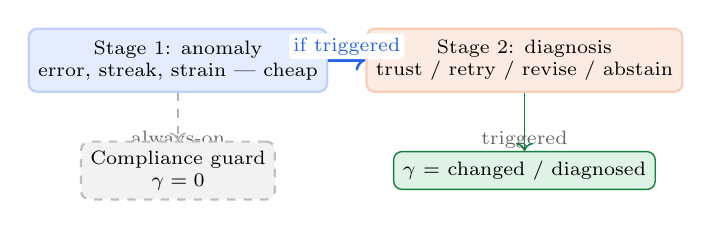
\begin{tikzpicture}[thick, every node/.style={font=\scriptsize}]
  \node[draw, rounded corners=3pt, fill=loopblue!12, draw=loopblue!30, minimum width=2.8cm, minimum height=0.80cm, align=center] (s1) at (-2.2,0) {Stage 1: anomaly\\{\scriptsize error, streak, strain — cheap}};
  \node[draw, rounded corners=3pt, fill=looporange!12, draw=looporange!30, minimum width=2.8cm, minimum height=0.80cm, align=center] (s2) at (2.2,0) {Stage 2: diagnosis\\{\scriptsize trust / retry / revise / abstain}};
  \draw[->, loopblue, line width=0.9pt] (s1) -- node[above, loop label small] {if triggered} (s2);
  \node[below=0.35cm of s1, font=\scriptsize, text=black!60, align=center] {always-on};
  \node[below=0.35cm of s2, font=\scriptsize, text=black!60, align=center] {triggered};
  \node[draw, rounded corners=3pt, fill=loopgreen!14, draw=loopgreenDark, line width=0.5pt, minimum width=1.9cm, align=center] (g) at (2.2,-1.4) {$\gamma$ = changed / diagnosed};
  \draw[->, loopgreenDark, line width=0.6pt] (s2.south) -- (g.north);
  \node[draw, dashed, rounded corners=3pt, fill=gray!10, draw=gray!50, minimum width=1.9cm, align=center] (cg) at (-2.2,-1.4) {Compliance guard\\{\scriptsize $\gamma=0$}};
  \draw[->, gray!60, dashed, line width=0.6pt] (s1.south) -- (cg.north);
\end{tikzpicture}
\caption{The $\gamma$-gate: slower loop vetoing faster one. Stage 1 (cheap, always-on) scores anomaly; Stage 2 (triggered) diagnoses and may change action. $\gamma$ measures whether watching steered. Compliance guard (identical reports, never consults policy) proves $\gamma=0$ is inert watching.}
\label{fig:gammagate}
\end{figure}

\textbf{And the deepest incompleteness --- the observer that watches the observer:} Energy hits 0.15 and nothing dies. This is the allostatic gap \citep{seth2021}: organisms whose essential variables must stay viable develop experience \emph{because} failure means dissolution --- ceasing to exist as organized systems. Until consequences are irreversible --- until the relations that make the system \emph{this} system scatter and cannot be reassembled as the same one --- the witness is evidentiary, not existential. Seth says stakes are not an addition to consciousness. They \emph{are} consciousness. Our \texttt{DissolutionError} is a gesture --- the agent scatters into survivors, reassembly produces a different agent. The 200-turn irreversible life is the test: does survival pressure create honesty? The question the witness makes testable is not ``is the agent conscious?'' but ``does the agent behave as if its claims matter for whether it continues to be \emph{this} agent?'' That is allostasis made measurable --- and the observer that watches whether stakes matter is itself the next slower loop, also constructed, also needing watching. Turtles all the way down, but each turtle can still veto the one above.


\textbf{Loops at every scale --- each could be its own paper:}

\textit{Molecule (BCM metaplasticity):} Quiet neurons lower $\theta_m$ (more plastic), hyperactive raise it (less) \citep{bienenstock1982}. Loop: activity $\to$\allowbreak{} threshold slides $\to$\allowbreak{} next activity's plasticity different $\to$\allowbreak{} next threshold slides differently. The synapse watches its own recent activity and vetoes its own next plasticity.

\textit{Circuit (efference copy):} Motor command copy sent to sensory cortex before movement, predicts sensory consequence, vetoes self-produced input as ``not external'' \citep{seth2021}. Loop: command $\to$\allowbreak{} copy $\to$\allowbreak{} predict $\to$\allowbreak{} compare to actual $\to$\allowbreak{} veto if self-caused. Without it, you can't tickle yourself --- prediction vetoes.

\textit{Mind (PFC veto):} Amygdala proposes threat $\to$\allowbreak{} PFC scores anomaly $\to$\allowbreak{} if triggered, diagnoses $\to$\allowbreak{} vetoes $\to$\allowbreak{} threat not acted on $\to$\allowbreak{} next threat proposal weaker \citep{seth2021,macar2026}. Loop: impulse $\to$\allowbreak{} watcher scores $\to$\allowbreak{} watcher diagnoses $\to$\allowbreak{} veto $\to$\allowbreak{} impulse not reinforced. Without it, worry spiral: one coalition wins forever.

\textit{Person (journal):} Day's behavior $\to$\allowbreak{} evening journal $\to$\allowbreak{} audit (what actually happened vs storied) $\to$\allowbreak{} next day's behavior different \citep{ghazali1106ihya}. Loop: act $\to$\allowbreak{} record $\to$\allowbreak{} audit $\to$\allowbreak{} next act checked against record. Without it, same story, same act, same story.

\textit{Harness ($\gamma$-gate):} Generation $\to$\allowbreak{} anomaly score $\to$\allowbreak{} if triggered, diagnose $\to$\allowbreak{} policy $\to$\allowbreak{} changed or not $\to$\allowbreak{} $\gamma$ measured \citep{macar2026,cao2026}. Loop: generate $\to$\allowbreak{} watcher scores $\to$\allowbreak{} watcher diagnoses $\to$\allowbreak{} watcher may veto $\to$\allowbreak{} next generation different. Without it, beautiful reports, zero steering.

\textit{Machine (shadow mode):} The ultimate observer at machine scale --- silent witness vs active actor. Tesla's shadow mode splits consciousness into two parallel tracks: the human driver physically steering and the autonomous software silently simulating what it \emph{would} do, outputs disconnected. Both receive the same sensor data; only the human acts. A comparison engine detects mismatches: if shadow predicts ``brake for pedestrian'' but human accelerates (sees pedestrian looking away), the 10-second clip is flagged for cloud training. This is efference copy at fleet scale: predicted trajectory vs actual, veto if self-caused. Loop: human act + shadow prediction $\to$\allowbreak{} mismatch detection $\to$\allowbreak{} cloud $\to$\allowbreak{} fleet-wide LTP (reinforce correct trajectory) or LTD (de-weight ghost obstacle via clathrin-like pruning). Without shadow mode, the AV has no observer --- generation directly drives actuation, no veto. Roundabout panic is what happens when the observer is present but too conservative: AV calculates gap $\to$\allowbreak{} inches forward $\to$\allowbreak{} safety harness vetoes (1\% collision risk) $\to$\allowbreak{} slams brakes $\to$\allowbreak{} human drivers honk and swerve $\to$\allowbreak{} sensors see escalated chaos $\to$\allowbreak{} safety envelopes shrink $\to$\allowbreak{} paralyzed in runaway indecision, where defensive actions create the chaos that justifies more defense. The AV's own veto creates the evidence for its next veto --- reflexive loop without damping, identical to a human panic attack.

\textit{Universe (awareness):} Measurement perturbs what it measures $\to$\allowbreak{} next measurement must be about perturbed world $\to$\allowbreak{} next theory must describe new world. Loop: observe $\to$\allowbreak{} world now contains observation $\to$\allowbreak{} next observation different. The observer at universe scale is the practice that sustains the loop being what it is at each instant.

\textbf{Harness:} \texttt{MonitorGate}: \texttt{DetectSignals} (error rate, failure streak, context conflict, embodied strain) $\to$\allowbreak{}\\ \texttt{evaluate()} $\to$\allowbreak{} \texttt{anomaly\_score} $\to$\allowbreak{} if triggered, \texttt{diagnose()} $\to$\allowbreak{} \texttt{policy} (trust/retry/revise/abstain) $\to$\allowbreak{} \texttt{override\_rate()} ($\gamma$) \citep{macar2026,cao2026}. Compliance guard as permanent negative control ($\gamma=0$ by construction). Every turn, cheap; only when triggered, expensive. The observer is not a module. It is the \emph{gating} that determines whether the next broadcast will be the winner's content or the veto's abstention. Each of these --- anomaly detection, diagnosis, policy selection, override measurement, and the allostatic gap that makes the observer matter --- carries enough open questions to be studied on its own.

\textbf{What it tells you to do:} Build the slower watcher and give it a record it can check before the next vote. Not a better narrator. A witness the narrator cannot edit, checked by a watcher slower than the narrator, whose checking is measured by whether it actually changed the next action. Journal outside the skull. Weekly review over daily habits. Ledger over claim. Sham over format. Counterfactual over actual. Dissolution over simulation. Turtles all the way down --- but each turtle's veto is the only agency the turtle above will ever have, and it is enough to change the loop, one veto at a time.

%==============================================================================
\section{How It All Works at Every Level}
\label{sec:levels}
%==============================================================================

One loop. Different substrates. How they interlock (Figure~\ref{fig:nested} shows the nesting: each level's broadcast is the next level's input, consolidation the next level's boundary, state the next level's bias):

\begin{center}
\small
\begin{tabular}{p{1.95cm}p{2.35cm}p{2.35cm}p{2.35cm}p{2.85cm}}
\toprule
Level & Boundary & Competition & Broadcast & Consolidation \\
\midrule
Molecule & Cleft & Big vs small Ca$^{2+}$ & CaMKII switch & Tag-and-capture \\
Cell & Membrane & Summation & Spike & STDP \\
Circuit & Hippo vs cortex & Salience tagging & Replay (10--20$\times$) & SHY + replay \\
Mind & Narrative self & 6--8 parties bid & Workspace & Light$\to$\allowbreak{}Deep \\
Person & Life story & Habit vs deliberation & Action & Character \\
Society & Legal entity & Buy vs sell & Price & Institutions \\
Harness & Ledger & Plugins bid & Workspace + spans & Light$\to$\allowbreak{}C.-factual$\to$\allowbreak{}Deep \\
Universe & System vs env & Theory vs theory & Law & Paradigm \\
\bottomrule
\end{tabular}
\end{center}

\begin{figure}[htbp]
\centering
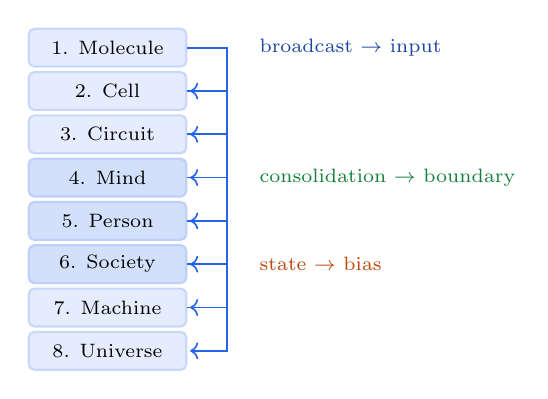
\begin{tikzpicture}[thick, every node/.style={font=\scriptsize}]
  \node[draw, rounded corners=2pt, fill=loopblue!12, draw=loopblue!25, minimum width=2.0cm, minimum height=0.48cm, align=center] (l1) at (0,3.4) {1. Molecule};
  \node[draw, rounded corners=2pt, fill=loopblue!12, draw=loopblue!25, minimum width=2.0cm, minimum height=0.48cm, align=center] (l2) at (0,2.85) {2. Cell};
  \node[draw, rounded corners=2pt, fill=loopblue!12, draw=loopblue!25, minimum width=2.0cm, minimum height=0.48cm, align=center] (l3) at (0,2.3) {3. Circuit};
  \node[draw, rounded corners=2pt, fill=loopblue!20, draw=loopblue!30, minimum width=2.0cm, minimum height=0.48cm, align=center] (l4) at (0,1.75) {4. Mind};
  \node[draw, rounded corners=2pt, fill=loopblue!20, draw=loopblue!30, minimum width=2.0cm, minimum height=0.48cm, align=center] (l5) at (0,1.2) {5. Person};
  \node[draw, rounded corners=2pt, fill=loopblue!20, draw=loopblue!30, minimum width=2.0cm, minimum height=0.48cm, align=center] (l6) at (0,0.65) {6. Society};
  \node[draw, rounded corners=2pt, fill=loopblue!12, draw=loopblue!25, minimum width=2.0cm, minimum height=0.48cm, align=center] (l7) at (0,0.1) {7. Machine};
  \node[draw, rounded corners=2pt, fill=loopblue!12, draw=loopblue!25, minimum width=2.0cm, minimum height=0.48cm, align=center] (l8) at (0,-0.45) {8. Universe};
  \foreach \i in {1,...,7} {
    \pgfmathtruncatemacro{\j}{\i+1}
    \draw[->, loopblue, line width=0.6pt, shorten >=1pt] (l\i.east) -- ++(0.5,0) |- (l\j.east);
  }
  \node[right=0.85cm of l1, font=\scriptsize, text=loopblue!70!black, fill=white, inner sep=1.5pt, rounded corners=1pt, align=left] {broadcast $\to$\allowbreak{} input};
  \node[right=0.85cm of l4, font=\scriptsize, text=loopgreenDark, fill=white, inner sep=1.5pt, rounded corners=1pt, align=left] {consolidation $\to$\allowbreak{} boundary};
  \node[right=0.85cm of l6, font=\scriptsize, text=looporange!80!black, fill=white, inner sep=1.5pt, rounded corners=1pt, align=left] {state $\to$\allowbreak{} bias};
\end{tikzpicture}
\caption{How the eight levels nest: each level's broadcast is the next level's input, consolidation is the next level's boundary, state is the next level's bias. One loop nested 8 times — not many loops like each other, but one loop at 8 scales.}
\label{fig:nested}
\end{figure}

How they interlock:
\begin{enumerate}
\item Each level's broadcast is the next level's input (spike $\to$\allowbreak{} circuit, replay $\to$\allowbreak{} cortex, thought $\to$\allowbreak{} action, action $\to$\allowbreak{} price, price $\to$\allowbreak{} paradigm). No level is closed. Every broadcast perturbs the next loop.
\item Each level's consolidation is the next level's boundary (LTP $\to$\allowbreak{} synapse strength $\to$\allowbreak{} circuit boundary; SHY $\to$\allowbreak{} cortex $\to$\allowbreak{} mind's memory; Light$\to$\allowbreak{}Deep $\to$\allowbreak{} semantic $\to$\allowbreak{} person's character). The slow memory of one level is the boundary of the next.
\item Each level's state update is the next level's competition bias (BCM $\theta_m \to$ synapse; adenosine $\to$\allowbreak{} circuit; energy/affect $\to$\allowbreak{} mind; character $\to$\allowbreak{} person; funding invariant $\to$\allowbreak{} market). Same five organs, different substrate.
\item Same five organs at every level because each faces the same problem: stable enough to persist while flexible enough to learn, in a world that contains itself, under uncertainty, over time, where every action perturbs the conditions for the next action.
\end{enumerate}

We now walk each level in turn. Every one is given as a numbered sequence, with the science that makes it checkable.

\subsection{Level 1: Molecule --- The Synapse (Ca$^{2+}$ as vote, AMPA as broadcast)}

\textit{Boundary:} Synaptic cleft (20\,nm) --- pre vs post, which side fired is whose responsibility, so coincidence can be detected \citep{tononi2014}. Without the cleft, no pre/post distinction, NMDA cannot detect coincidence, Hebb fails.

\textit{The loop, step by step.}
\begin{enumerate}\itemsep2pt
\item \textbf{Two things must happen at once.} Glutamate arrives from the
presynaptic side, \emph{and} the postsynaptic side is already depolarized
(which ejects the Mg$^{2+}$ plug; glycine must also be present). Only then
does the NMDA receptor open. This is what makes it a coincidence detector:
one signal alone does nothing.
\item \textbf{Calcium enters, and its shape decides the outcome.} A large,
brief Ca$^{2+}$ spike flips the CaMKII Thr286 switch --- each subunit
phosphorylates its neighbour, so the switch stays on after the calcium has
cleared. That is a molecular memory of an event that has already ended.
\item \textbf{The synapse gets stronger.} More AMPA receptors are inserted,
so the same input produces a larger response next time.
\item \textbf{A stronger synapse is more likely to fire with its partner
again}, more likely to push the cell over threshold, and therefore more
likely to be strengthened again. The loop amplifies itself \citep{tononi2014}.
\end{enumerate}

Three mechanisms keep that amplification from running away or firing
indiscriminately. Salience decides which synapses get the scarce proteins:
a large Ca$^{2+}$ signal together with dopamine or noradrenaline sets the
tag that captures them. The BCM threshold $\theta_m$ slides with the
neuron's own recent history, so a hyperactive neuron becomes harder to
potentiate \citep{bienenstock1982}. Oja's rule normalizes the weights so
no single input can take all the strength \citep{oja1982}. Perineuronal
nets act as a write-protect flag on what has already been learned.

The synapse is therefore already a reflexive loop in miniature: its
current strength determines whether the next coincidence is detected at
all, and that detection determines its next strength.

\subsection{Level 2: Cell --- The Neuron (firing as vote, network as workspace)}

\textit{Boundary:} Cell membrane, self-produced: metabolism builds the lipids that self-assemble into the membrane that bounds the metabolism \citep{maturana1980}. No membrane, no cell; no network, no membrane. The neuron persists as a pattern, not as stuff --- proteins turn over in days, the network regenerates \citep{maturana1980}. This is autopoiesis at cellular scale: the cell is the first reflexive loop at the scale of life.

\textit{The loop, step by step.}
\begin{enumerate}\itemsep2pt
\item \textbf{Thousands of synapses vote.} Each input is a vote for
``fire'' or ``don't,'' and no single one is decisive.
\item \textbf{The votes are summed in space and time} at the axon hillock.
Inputs that arrive together count for more than the same inputs spread out
--- coincidence wins.
\item \textbf{One all-or-nothing spike is broadcast} to every downstream
synapse. There is no partial answer and no private answer.
\item \textbf{Firing changes who will be talking next time.} Which
presynaptic partners stay active depends on what just fired, so the next
vote is taken among a different set of voters \citep{white1986,dorkenwald2023}.
\end{enumerate}

Timing decides the direction of the change: when the presynaptic cell
fires \emph{before} the postsynaptic one the connection strengthens, and
when it fires after, the connection weakens \citep{bipoo1998}. That
asymmetry is how a network turns mere correlation into something closer to
causation. After-hyperpolarization adapts the threshold, and
neuromodulators shift the gain of the whole cell at once.

A neuron, then, is a parliament of synapses competing for a single
broadcast. No individual synapse decides. The configuration votes.

\subsection{Level 3: Circuit --- Hippocampus and Cortex (fast vs slow as two parliaments)}

\textit{Boundary:} Hippocampus vs cortex --- which memories are where, pattern-separated (hippocampus, one-shot, distinct) vs statistical (cortex, interleaved) \citep{tononi2014}. This boundary is not anatomical only. It is functional: two parliaments with different rules, competing for consolidation priority.

\textit{The loop, step by step.}
\begin{enumerate}\itemsep2pt
\item \textbf{Experience is tagged, not stored.} Not everything survives
the day. Salience --- emotion, surprise, prediction error --- decides which
traces are marked for consolidation \citep{seth2021}.
\item \textbf{The tagged traces are replayed during sleep.} Hippocampal
ripples, nested inside spindles, nested inside slow waves, replay the day
at 10--20$\times$ compression \citep{tononi2014}.
\item \textbf{Two operations run at night, not one.} Global downscaling
multiplies every synapse by a factor below one, which keeps the relative
strengths and deletes the noise; replay writes the surviving patterns into
cortex \citep{tononi2014}. Adenosine is the receipt for the day's
potentiation; perineuronal nets write-protect what is already settled; the
BDNF available for the whole process is budgeted by exercise and stress.
\item \textbf{The consolidated cortex changes what the next day can even
recognize.} Perception is filtered through what was kept.
\end{enumerate}

Skip the save and the day's tagging is wasted: potentiation saturates, and
a network that has learned everything distinguishes nothing.

Two-speed memory at circuit scale, fast labile vs slow structural, with sleep as the save. The circuit is an enactive loop: it doesn't store the world, it brings forth the world its loops can distinguish, and then must distinguish the world it just brought forth \citep{maturana1980}.

\subsection{Level 4: Mind --- The Parliament (coalition as vote, workspace as broadcast)}

\textit{Boundary:} the narrative self (L6) --- the line between ``this
story is mine'' and ``that story was handed to me.'' Four properties make
that line hold. Revisions are \emph{compare-and-set}: an update must claim
revision $N{+}1$ against the current $N$ or it is rejected, so no two
writers can silently overwrite each other. Every revision is
\emph{cause-signed} by one of three channels --- the agent updating itself
from a tool result, a compaction rewriting the story, or a direct human
write --- so a trait the narrator merely asserted can never be filed as
one the agent actually lived. Each version is \emph{archived verbatim} and
therefore diffable. And the story is \emph{re-injected every turn},
because a persona left to context position alone drifts more than 30\%
within twelve turns \citep{choi2024}. The self is not stored. It is
performed.

\textit{The loop, step by step.}
\begin{enumerate}\itemsep2pt
\item \textbf{Proposals arrive with bids.} Sensory input, body state,
memory, and affect each put forward a candidate for what happens next.
Each bid is roughly salience $\times$ utility --- how much this demands
attention, times how useful it looks.
\item \textbf{Six to eight parties compete for one microphone.}
Perception, memory, body budget, affect, habit, planner, and narrator all
bid, and a new vote runs roughly every 200\,ms
(Figure~\ref{fig:parliament}) \citep{baars1997,atallah2026gwt}.
Neuromodulators set the rules of that election: noradrenaline sets the
volume, dopamine sets the stake, and valence sets the risk dial
\citep{sofroniew2026}.
\item \textbf{The winner is broadcast to everyone at once.} Every
specialist gets the winning content simultaneously \citep{baars1997}. You
experience this broadcast as ``my thought.''
\item \textbf{Winning is rehearsed, and rehearsal is physical.}
Repetition myelinates the pathway, and a myelinated pathway conducts up to
100 times faster. Overnight, the day's traces run the consolidation
pipeline (Light $\to$ REM $\to$ Counterfactual $\to$ Deep), where every
promotion must carry a signed cause or it is blocked.
\item \textbf{The body pays for the turn.} Energy drains toward its floor,
fatigue rises toward its cap, and valence and arousal shift --- all of
which change the bids in the next round \citep{seth2021}.
\item \textbf{The broadcast becomes the next context.} Nothing resets. The
next competition begins inside the world the last one produced, and the
coalition that just won is now more likely to win again. That is the
difference between a footpath and a highway.
\end{enumerate}

The mind is not a thing that \emph{has} a parliament. The mind \emph{is}
that competition, broadcast and then rehearsed. There is no captain; the
configuration votes. And the narrator wins \emph{after} the action, then
explains as though it had decided
\citep{gazzaniga2000,johansson2005,nisbett1977}.

\begin{figure}[htbp]
\centering
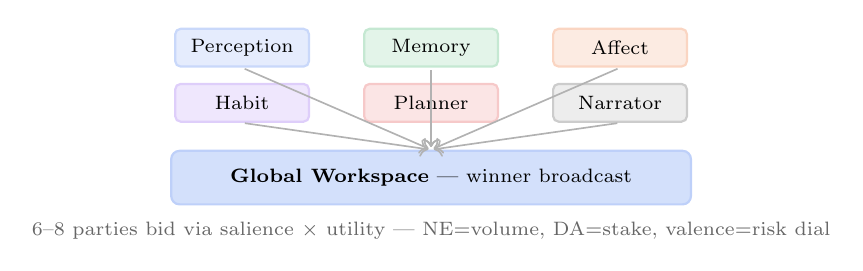
\begin{tikzpicture}[thick, every node/.style={font=\scriptsize}]
  \node[draw, rounded corners=2pt, fill=loopblue!12, draw=loopblue!25, minimum width=1.70cm, minimum height=0.48cm, align=center] (p) at (-2.4,1.0) {Perception};
  \node[draw, rounded corners=2pt, fill=loopgreen!12, draw=loopgreen!25, minimum width=1.70cm, minimum height=0.48cm, align=center] (m) at (0,1.0) {Memory};
  \node[draw, rounded corners=2pt, fill=looporange!12, draw=looporange!25, minimum width=1.70cm, minimum height=0.48cm, align=center] (a) at (2.4,1.0) {Affect};
  \node[draw, rounded corners=2pt, fill=looppurple!12, draw=looppurple!25, minimum width=1.70cm, minimum height=0.48cm, align=center] (h) at (-2.4,0.3) {Habit};
  \node[draw, rounded corners=2pt, fill=loopred!12, draw=loopred!25, minimum width=1.70cm, minimum height=0.48cm, align=center] (pl) at (0,0.3) {Planner};
  \node[draw, rounded corners=2pt, fill=gray!14, draw=gray!40, minimum width=1.70cm, minimum height=0.48cm, align=center] (n) at (2.4,0.3) {Narrator};
  \node[draw, rounded corners=3pt, fill=loopblue!20, draw=loopblue!30, minimum width=6.6cm, minimum height=0.68cm, align=center] (ws) at (0,-0.65) {\textbf{Global Workspace} — winner broadcast};
  \foreach \src in {p,m,a,h,pl,n} \draw[->, gray!60, line width=0.6pt, shorten >=1pt, shorten <=1pt] (\src.south) -- (ws.north);
  \node[below=0.14cm of ws, font=\scriptsize, text=black!60, align=center, fill=white, inner sep=1.5pt, rounded corners=1pt] {6--8 parties bid via salience $\times$ utility — NE=volume, DA=stake, valence=risk dial};
\end{tikzpicture}
\caption{The parliament at mind scale: 6 parties bid via salience $\times$ utility; winner broadcast globally, experienced as ``my thought'' 200\,ms after competition. No captain, configuration votes. This is Layer 4, the global workspace where coalition competition becomes conscious access.}
\label{fig:parliament}
\end{figure}

\subsection{Level 5: Person --- The Life (choice as vote, story as broadcast)}

\textit{Boundary:} Life story --- ``this is who I am over time'' vs ``that was something that happened to me'' --- maintained narrative, not stored fact. The boundary is the story that persists because it is re-injected, or it ceases. Same as the synapse's boundary, but at the scale of a life.

\textit{The loop, step by step.}
\begin{enumerate}\itemsep2pt
\item \textbf{The situation arrives already filtered.} What the world
presents has passed through your affordances first. An exhausted self does
not face a harder choice; it faces \emph{fewer options}, because the
tiring ones never appear as candidates \citep{seth2021}.
\item \textbf{Habit, deliberation, affect, and social expectation bid
against each other} --- and your state rigs the vote before it starts.
Tired and anxious is a different parliament from rested and safe, running
on the same hardware.
\item \textbf{You act, and the act enters the world.} It is now a
consequence other people and future situations must respond to.
\item \textbf{You are a different person perceiving a different world.}
The record, the self-model, and the skills have all changed; so has what
they are looking at.
\item \textbf{You replay what happened, then what could have happened.}
The counterfactual produces regret, and regret is the gradient --- a
simulation of yourself in the world, run to calibrate the next turn
\citep{tononi2014,sofroniew2026}.
\item \textbf{Character accumulates as an attractor}: which coalitions
tend to win, carved by every rehearsal that came before.
\end{enumerate}

The loop widens and never returns to where it started. A life is not a
thing that has a self that has loops. A life \emph{is} the expanding
reflexive loop that, by looping, produces the experience of being someone
who has it \citep{maturana1980}.

\subsection{Level 6: Society --- The Market (order as vote, price as broadcast)}

\textit{Boundary:} Legal entity, balance sheet --- this capital is mine, that liability is yours, who bears exhaustion risk when the money runs out. No legal boundary $\to$\allowbreak{} risk socialized, loops feed without bound, no accountability --- Spring-Loaded Door where institutional anchors are cut and loops spring, feeding on whatever is nearby. Each market is a paper: legal entity as boundary, balance sheet as ledger.

\textit{The loop, step by step.}
\begin{enumerate}\itemsep2pt
\item \textbf{Information perturbs the price.} News, order flow, and
belief all arrive as candidates for what the asset is worth.
\item \textbf{Buyers and sellers bid, and so do narratives.} The weight
behind a story is its salience (volume, attention, coverage) times its
utility (expected risk-adjusted return). The order book is where those
bids are resolved.
\item \textbf{The price is broadcast to every participant at once} --- and
immediately becomes the reality that every subsequent decision has to
respond to.
\item \textbf{Institutions, law, and culture are the slow memory}: they
encode which competitions have tended to win, and they persist long after
the trades that made them.
\item \textbf{Damping is deliberate and institutional}: funding
invariants, kill criteria, position limits, circuit breakers, a central
bank. Remove them and the loop has no brake.
\end{enumerate}

The price is the prediction, and the prediction is the price: belief
creates the reality the belief was about \citep{soros1987}. Soros's two
functions --- understanding reality and changing it --- run simultaneously,
and neither yields a determinate answer alone. No single trader decides.
The configuration of beliefs, weighted by capital and salience, votes.

\subsection{Level 7: Machine --- The Harness (plugin as vote, ledger as broadcast)}

\textit{Boundary:} Provenance Ledger (L1) --- every span carries source\-\\$\in\{$memory\_lookup, model\_prior, monitor\_override, external-tool$\}$ + ref --- inside vs outside, what to trust, what to check \citep{gazzaniga2000,johansson2005}. Without it, claims float free, S126 failure: 98\% confidence on fabrications vs 87\% on truths --- more confident about lies than truth.

\textit{The loop, step by step.}
\begin{enumerate}\itemsep2pt
\item \textbf{Proposals arrive with bids}, exactly as in the mind: the
prompt, body signals, memory, and affect each put forward a candidate,
weighted by salience $\times$ utility.
\item \textbf{Plugins bid --- and they need not share a model.} Perception
can be a VLM, memory a retrieval model, affect a steered model, the
planner a reasoner, habit a skill model, and the narrator a press
secretary; each carries its own weights, prompt, and temperature
\citep{lin2026ahe}. Many tongues, one harness.
\item \textbf{The workspace scores the bids}, with AffectState scaling
them within a bounded range, and one winner is broadcast --- together with
its provenance spans, so the broadcast is auditable rather than merely
available \citep{baars1997,atallah2026gwt}.
\item \textbf{The model's next input is its own last output, plus the
ledger.} That second term is the whole difference
\citep{lindsey2025,macar2026}.
\item \textbf{Consolidation runs offline} (Light $\to$ REM $\to$
Counterfactual $\to$ Deep), and an untagged promotion is blocked outright.
\item \textbf{The body and the observer both keep score.} Energy drains
toward its floor, fatigue rises toward its cap, and $\gamma$ records
whether diagnosis actually changed the action.
\item \textbf{State($t$) becomes harness($t{+}1$).} The harness rewrites
the conditions for its own next iteration \citep{maturana1980}.
\end{enumerate}

Remove the ledger and step 4 collapses into a hallucination loop: the
model generates, reads its own output back as context, predicts a
continuation consistent with itself, and generates more of the same. There
is no outside. The ledger \emph{is} the outside.

\subsection{Level 8: Universe --- The Reflexive Whole (measurement as vote, law as broadcast)}

\textit{Boundary:} What counts as system vs environment --- observer vs observed (but observer is made of what it observes) \citep{maturana1980}. Holographic principle (information on boundary), cosmological horizon (observable limit), decoherence (where facts get bound) as candidates. The boundary is where facts become definite enough to be recorded --- where the loop's prediction becomes checkable.

\textit{The loop, step by step.}
\begin{enumerate}\itemsep2pt
\item \textbf{Measurement makes a property definite.} Any interaction that
settles what was previously open counts.
\item \textbf{Descriptions compete.} Theory against theory, instrument
against instrument, weighted by salience (precision, funding, attention)
and utility (predictive power).
\item \textbf{The winner is broadcast as law} --- ``how the universe
works'' --- and becomes the thing every subsequent measurement is designed
to be about.
\item \textbf{Paradigm is the slow memory} that encodes which competitions
have tended to win.
\item \textbf{The next description must describe a world the last one
already changed}, because a theory that is believed and acted on alters
what there is to describe.
\end{enumerate}

This is the same loop as every level above, at the scale where system and
world are no longer separable even in principle: the map becomes part of
the territory. Not mysticism --- reflexivity, taken to its limit.

One process at that scale, with an audit trail that lets the slower watcher check the faster loop before the next vote. Change what you feed the loop and whether the watcher can check, at any scale, and you change what the loop becomes at every scale above it.

%==============================================================================
\subsection{Prior observational taxonomies}
\label{sec:traditions}

Several contemplative traditions produced detailed taxonomies of mind from
sustained first-person observation, and a number of their distinctions
correspond loosely to the five organs: Abhidharma's list of mental factors
co-arising in varying subsets resembles a competition among specialists;
Sufism's distinction between a retained station and a transient state
resembles two-speed memory; Stoic journalling is an external record checked
against recalled behaviour.

We report these as historical context, not as evidence. The correspondences
are ours, they are loose, and no weight in this paper rests on them --- the
claims in \S\ref{sec:organs} stand or fall on the ablations in
\S\ref{sec:falsifiability}. We note them only because a reader may wonder
whether the five-organ decomposition is arbitrary; the fact that independent
observers carving up the same territory reached broadly similar distinctions
is weak evidence that it is not, and nothing stronger.

\begin{center}
\setlength{\tabcolsep}{3pt}
\small
\begin{tabular}{P{2.4cm}P{3.4cm}P{5.6cm}}
\toprule
Tradition & Method & Distinction it recorded \\
\midrule
Abhidharma & First-person observation, catalogued over centuries & Mental factors co-arising in varying subsets \\
Sufism & Staged practice under supervision & Retained stage vs transient state \\
Advaita & Systematic negation & Appearance vs what survives negation \\
Stoicism & Daily written record; rehearsing adverse cases & What is and is not within one's control \\
Phenomenology & Disciplined description, suspending interpretation & Lived body as precondition for perception \\
\bottomrule
\end{tabular}
\end{center}

\subsection{A note on scope}
\label{sec:universe}

The scales in \S\ref{sec:levels} run from the synapse to the market. We stop
there. It is tempting to extend the argument to physical cosmology --- to ask
what plays the role of a boundary or a damping term for the universe as a
whole --- and earlier drafts of this paper did so. We have removed that
material. The five-organ account earns its keep only where the ablations in
\S\ref{sec:falsifiability} can actually be run, and at cosmological scale they
cannot. Extending the framework there would make it unfalsifiable in exactly
the way the rest of this paper is designed to avoid.

%==============================================================================
\section{The Only Real Choice}
\label{sec:choice}
%==============================================================================

What you feed the loop and whether the slower watcher can check the record before the next vote. This is not poetry. It is the operational conclusion:

\begin{itemize}
\item \textbf{What you feed the loop} is the salience gate, the rehearsal, the myelination. Worry practiced 1,000 times builds elite worry circuits --- 100$\times$ conduction speed for whatever you repeat.
\item \textbf{Whether the watcher can check} is the witness, the $\gamma$-gate, the sham control. Checkability is enough, because the narrator's story, told often enough and never checked, becomes the highway.
\end{itemize}

You don't choose the options --- affordance gating removes some before they appear. You don't fully choose the winner --- the parliament votes without a captain, 200ms before you feel you chose. You can veto the winner, keep a witness that makes the next winner more honest, and slowly change which options appear by what you rehearse. That is not the free will you were promised. It is the free will you actually have, and it is enough if you use it where it lives.

\begin{center}
\begin{tabular}{p{5.7cm}p{5.7cm}}
\toprule
Pick what you rehearse --- myelination keeps the receipt & Externalize the witness --- write \\
Protect sleep --- global downscaling + 10--20$\times$ replay & Never let a fast loop grade its own homework \\
Buy BDNF with exercise --- lactate $\to$\allowbreak{} BDNF $\to$\allowbreak{} mTORC1 & You don't choose whether to feed the loop \\
& --- only what you feed it \\
\bottomrule
\end{tabular}
\end{center}

%==============================================================================
\section{Falsifiability}
\label{sec:falsifiability}
%==============================================================================

The five-organ claim is falsifiable by ablation at any scale, and we state the verbatim selection pressures so the mapping can be checked. \emph{Our mapping} of Nayebi Cor.~3--5 to the five organs (boundary, two-speed memory, salience gate, damping, internal observer) is an executable interpretation, not Nayebi's terminology; see Appendix for verbatim Corollaries. If the mapping is wrong, the ablation predicted to fail will not fail, and the paper is wrong in a checkable way.

\begin{center}
\small
\begin{tabular}{p{2.2cm}p{3.8cm}p{3.8cm}p{3.8cm}}
\toprule
Organ & Synapse ablation & Circuit ablation & Harness ablation \\
\midrule
Boundary & Remove cleft $\to$\allowbreak{} no Hebb & Lesion perirhinal $\to$\allowbreak{} no recognition & Remove ledger $\to$\allowbreak{} 98\% on fabrications \\
Two-speed & Block late LTP $\to$\allowbreak{} no consolidation & Lesion hippocampus $\to$\allowbreak{} no one-shot & Ablate Light/REM/Deep: each carries work \\
Salience & Block DA/NE $\to$\allowbreak{} no tagging & Blunt affect $\to$\allowbreak{} no distinction & Remove AffectState $\to$\allowbreak{} saturation \\
Damping & Block LTD/BCM $\to$\allowbreak{} seizure & Block SHY $\to$\allowbreak{} saturation & Remove cull\_failed $\to$\allowbreak{} hallucination loop \\
Observer & Block efference copy $\to$\allowbreak{} can't tickle & Lesion PFC $\to$\allowbreak{} no veto & Set $\gamma=0$ (compliance guard) $\to$\allowbreak{} beautiful reports, zero steering \\
\bottomrule
\end{tabular}
\end{center}

Each cell is a prediction: ablate this organ at this scale and the pathology in \S\ref{sec:organs} appears. If it does not, the mapping is wrong for that scale, and the paper's claim is falsified at that cell. The harness makes the same test executable: ablate one organ, keep four, measure whether the predicted pathology appears (coverage, $\gamma$, promotion rate, skill survival, dissolution progress). This is why the audit trail matters: without it, falsifiability is assertion; with it, each ablation is a checkable prediction.

%==============================================================================
\section{What It All Means}
\label{sec:what-it-all-means}
%==============================================================================

It means the same answer appeared from four different directions, and we built the one place where they can be measured together.

\textit{Evolution} gave the worm 302 neurons wired as distributed local modules negotiating, not a central controller commanding \citep{white1986}. \textit{Connectomics} confirmed it at 140,000 neurons in the fly --- same surprise: local circuits control themselves, brain negotiates \citep{dorkenwald2023}. \textit{Mathematics} (Nayebi, UAI 2026) proved it must be so: any competent agent under mixed tasks is forced to develop the five --- or a task distribution will exploit the gap \citep{nayebi2026}. Cor.~5 says all such agents converge to the same partitions. \textit{Engineering} built it as a harness you can run: 11 modules, 8 layers, 78/78 green, with an audit trail for every thought. Four methods. One destination. That's not analogy. That's convergent validity.

What it means, concretely, is four things that are not separate:

\textbf{The harness is not a better prompt.} It is a different kind of thing: a mind made of relations, not a model made of weights. Change the relations (Cordis re-ties the cord every turn: $\mathrm{State}(t) \to \mathrm{harness}(t{+}1)$) and the same frozen LLM becomes a different agent \citep{lin2026ahe}. The loom is standard; the warp is mandatory; the weft is yours.

\textbf{The witness is the difference between intelligence and honesty.} Intelligence is producing good outputs. Honesty is knowing where they came from and being checkable about it. Without a ledger, 98\% confidence on fabrications vs 87\% on truths --- more confident about lies \citep{gazzaniga2000}. With a ledger no one checks, always-no (0.667). With a ledger that is checked, on a capable subject, 1.000. The EU just made provenance law and is learning watermarking $\neq$ ledger. Our sham control is the experiment that will tell whether content matters beyond format.

\textbf{You are the maintenance, not the moment.} Now is a 200\,ms stitched win\-dow \citep{libet1983,wegner2002}, self is a pattern re-injected every turn or it drifts 30\% in 12 \citep{choi2024}, world is a controlled hallucination \citep{seth2021,clark2016surfing}. None are found; all are performed. Agency is not choosing at now from a neutral menu --- the menu was rigged by what you rehearsed. It is the veto, the witness kept between nows, and the highway you pave by what you replay. The counterfactual we just wired (variant $\to$\allowbreak{} simulate through self-containing world model $\to$\allowbreak{} regret) is that maintenance made executable \citep{tononi2014}.

\textbf{Stakes are still missing.} Energy hits 0.15 and nothing dies. Seth's thesis says that's why the harness is still evidentiary, not existential \citep{seth2021}. The 200-turn irreversible life --- where ceiling only goes down, skills delete permanently, dissolution scatters the configuration --- is the test that makes the witness matter for whether the agent continues to be \emph{this} agent. Until then, the harness can be honest. With stakes, it would have a reason to care.

What it means for being human in such a universe is not that we are illusions and therefore nothing matters. It is that we are maintained illusions and therefore \emph{everything about maintenance matters} --- what you rehearse, whether you protect sleep, whether you keep a witness. That's what it all means: one loop at every scale, five organs at every level, and the only real choice is what you feed the loop and whether the slower watcher can check the record before the next vote. Everything else --- parliament of models, many tongues one harness, the chemical connectome --- is that same loop, woven tighter.

%==============================================================================
\section{Conclusion}
\label{sec:conclusion}
%==============================================================================

The dynamic reflexive loop and its five organs appear at every scale we can measure, were discovered by every tradition that watched long enough, and can now be built and measured in code with an audit trail. The harness is not a model of the mind. It is the mind's method --- and the synapse's, the market's, and perhaps the universe's --- made executable at one scale, with a record the next scale can check.

The boulder rolls downhill because gravity was always there. We didn't invent the war between subsystems, or the replay, or the need for a witness. We built the loom that can weave them and showed that the fabric it produces can be honest about where it came from, or not, depending on whether the witness is checked.

\begin{center}
\textit{One loop at every scale, five organs at every level, and the only real choice is what you feed the loop and whether the slower watcher can check the record before the next vote. Everything else is that same loop, woven tighter.}
\end{center}

\appendix
\section{Cordis Mapping: Eight Layers onto a Programmable Harness}
\label{app:cordis}

DeepSeek Harness (Cordis) is the loom: a kernel that mounts/unmounts plugins as reversible effects on a shared context. Every capability is a plugin; a profile composes bundles. MindHarness is one opinionated weave: five invariants as mandatory warp, each as a Cordis plugin with a metric, plus the audit trail. Fig.~\ref{fig:fivecycle} is our mapping of Nayebi Cor.~3--5, not Nayebi's figure.

\section{Verbatim Selection Pressures (Nayebi Cor.~3--5)}
\label{app:nayebi}

We quote the selection pressures verbatim so the mapping can be checked. Nayebi proves abstract pressures; the five-organ labeling (boundary, two-speed memory, salience gate, damping, internal observer) is our executable interpretation:

\textit{Corollary 3 (informational modularity):} Block-structured tasks force block-structured internal representations.

\textit{Corollary 4 (regime-tracking variables):} Under task mixtures, persistent regime-tracking variables resembling functional emotion primitives are forced.

\textit{Corollary 5 (representational convergence):} Under minimality, capable agents on shared tasks converge to shared decision-relevant partitions up to invertible recoding.

If the mapping of these pressures to the five organs is wrong for a scale, the ablation in \S\ref{sec:falsifiability} predicted to fail will not fail, and the paper is wrong in a checkable way. This is the falsifiability we claim, not immunity.

%==============================================================================
\bibliographystyle{plainnat}
\begin{thebibliography}{99}

\bibitem[Nayebi 2026]{nayebi2026}
Nayebi, A. (2026). What Capable Agents Must Know: Selection Theorems for Robust Decision-Making under Uncertainty. UAI 2026. arXiv:2603.02491. Verbatim Cor.~3--5 quoted in Appendix~\ref{app:nayebi}.

\bibitem[Lin et al. 2026]{lin2026ahe}
Lin, J., et al. (2026). Agentic Harness Engineering. arXiv:2604.25850.

\bibitem[Seth 2021]{seth2021}
Seth, A. (2021). \emph{Being You: A New Science of Consciousness}. Faber.

\bibitem[Tononi \& Cirelli 2014]{tononi2014}
Tononi, G., Cirelli, C. (2014). Sleep and the Price of Plasticity. \emph{Neuron}, 81, 12--34.

\bibitem[Nisbett \& Wilson 1977]{nisbett1977}
Nisbett, R., Wilson, T. (1977). Telling more than we can know. \emph{Psychological Review}, 84(3), 231--259.

\bibitem[Libet et al. 1983]{libet1983}
Libet, B., et al. (1983). Time of conscious intention to act. \emph{Brain}, 106(3), 623--642.

\bibitem[Wegner 2002]{wegner2002}
Wegner, D. (2002). \emph{The Illusion of Conscious Will}. MIT Press.

\bibitem[Gazzaniga 2000]{gazzaniga2000}
Gazzaniga, M. (2000). Cerebral specialization and interhemispheric communication. \emph{Brain}, 123, 1293--1326.

\bibitem[Choi et al. 2024]{choi2024}
Choi, J., et al. (2024). Examining Identity Drift in Conversations of LLM Agents. arXiv:2412.00804.

\bibitem[Panickssery et al. 2024]{panickssery2024}
Panickssery, N., et al. (2024). LLM Evaluators Recognize and Favor Their Own Generations. NeurIPS.

\bibitem[Macar et al. 2026]{macar2026}
Macar, U., et al. (2026). Mechanisms of Introspective Awareness. arXiv:2603.21396.

\bibitem[Sofroniew et al. 2026]{sofroniew2026}
Sofroniew, N., et al. (2026). Emotion Concepts and their Function in a Large Language Model. Anthropic.

\bibitem[Maturana \& Varela 1980]{maturana1980}
Maturana, H., Varela, F. (1980). \emph{Autopoiesis and Cognition}. Reidel.

\bibitem[White et al. 1986]{white1986}
White, J., et al. (1986). The structure of the nervous system of \emph{C. elegans}. \emph{Phil. Trans. R. Soc. B}, 314, 1--340.

\bibitem[Dorkenwald et al. 2023]{dorkenwald2023}
Dorkenwald, S., et al. (2023). FlyWire: brain-wide connectome of \emph{Drosophila}. \emph{Nature}, 634, 230--236.

\bibitem[Baars 1997]{baars1997}
Baars, B. (1997). In the Theater of Consciousness. Oxford UP.

\bibitem[Atallah 2026]{atallah2026gwt}
Atallah, S., et al. (2026). Design and Evaluation of a Global Workspace Agent
Embodied in a Realistic Multimodal Environment.
\emph{Frontiers in Computational Neuroscience}.

\bibitem[Cao et al. 2026]{cao2026}
Cao, Q., et al. (2026). LLMs Know When They Know, but Do Not Act on It:
A Metacognitive Harness for Test-time Scaling. arXiv:2605.14186.

\bibitem[Johansson et al. 2005]{johansson2005}
Johansson, P., et al. (2005). Choice blindness. \emph{Science}, 310, 116.

\bibitem[Lindsey 2025]{lindsey2025}
Lindsey, J. (2025). Emergent Introspective Awareness. Transformer Circuits.

\bibitem[Cacioli 2026]{cacioli2026}
Cacioli, J.-P. (2026). Do LLMs Know What They Know? Measuring Metacognitive
Efficiency with Signal Detection Theory. arXiv:2603.25112.

\bibitem[Maniscalco \& Lau 2012]{maniscalco2012}
Maniscalco, B., Lau, H. (2012). Signal detection theory for metacognition. \emph{Nature Neuroscience}, 15, 950--951.

\bibitem[Clark 2016]{clark2016surfing}
Clark, A. (2016). \emph{Surfing Uncertainty}. Oxford UP.

\bibitem[Al-Ghazali 1106]{ghazali1106ihya}
Al-Ghazali, A.H. (1106). \emph{I\d{h}y\=a' `Ul\=um al-D\=in} (Revival of the Religious Sciences). 40 books.

\bibitem[Paper v2 2026]{paper-v2-final}
Ahmed, S., et al. (2026). Witnessed Introspection in Assembled Language-Agent Systems (v2, 21pp, 10 figures, preregistered SHA-256 locks). MindHarness, tagged \texttt{paper-\allowbreak{}v2-\allowbreak{}final}, \texttt{github.com/\allowbreak{}shehzadahmed-\allowbreak{}xx/\allowbreak{}mindharness}.

\bibitem[Bienenstock et al. 1982]{bienenstock1982}
Bienenstock, E., Cooper, L., Munro, P. (1982). Theory for the development of neuron selectivity. \emph{J. Neuroscience}, 2, 32--48.

\bibitem[Oja 1982]{oja1982}
Oja, E. (1982). Simplified neuron model as a principal component analyzer. \emph{J. Math. Biology}, 15, 267--273.

\bibitem[Bi \& Poo 1998]{bipoo1998}
Bi, G., Poo, M. (1998). Synaptic modifications in cultured hippocampal neurons. \emph{J. Neuroscience}, 18, 10464--10472.

\bibitem[Pizzorusso et al. 2002]{pizzorusso2002}
Pizzorusso, T., et al. (2002). Reactivation of ocular dominance plasticity in the adult visual cortex. \emph{Science}, 298, 1248--1251.

\bibitem[Kandel 2001]{kandel2001}
Kandel, E. (2001). The molecular biology of memory storage. \emph{Science}, 294, 1030--1038.

\bibitem[Merzenich et al. 1984]{merzenich1984}
Merzenich, M., et al. (1984). Somatosensory cortical map changes following digit amputation in adult monkeys. \emph{J. Comp. Neurology}, 224, 591--605.

\bibitem[Paper v3 2026]{paper-v3}
Ahmed, S., et al. (2026). The Dynamic Reflexive Harness: Five Invariants from Molecules to Markets to Machines (v3, 29pp, App.\ A Cordis + App.\ B Mirror). MindHarness, \texttt{github.com/\allowbreak{}shehzadahmed-\allowbreak{}xx/\allowbreak{}mindharness}.

\bibitem[Giddens 1991]{giddens1991}
Giddens, A. (1991). \emph{Modernity and Self-Identity: Self and Society in the
Late Modern Age}. Polity Press.

\bibitem[Soros 1987]{soros1987}
Soros, G. (1987). \emph{The Alchemy of Finance}. Simon \& Schuster.

\bibitem[Fleming 2024]{fleming2024}
Fleming, S.M. (2024). Metacognition and Confidence: A Review and Synthesis.
\emph{Annual Review of Psychology}, 75, 241--268.

\end{thebibliography}

\end{document}
